\documentclass[11pt, a4paper]{article}
\usepackage[utf8]{inputenc}
\usepackage[left=2.35cm, right=3.35cm, top=3.35cm, bottom=3.0cm]{geometry}
\usepackage{amsmath, amssymb, amsthm}
\usepackage[english]{babel}
\usepackage{graphicx}
\usepackage[font={small,it}]{caption}
\graphicspath{ {figures/} }
\usepackage{url}
\usepackage{appendix}
\usepackage{float}
\usepackage{multirow}
\usepackage[bottom]{footmisc}
\usepackage{titling}
\usepackage{subcaption}
\usepackage{wrapfig}
\usepackage[numbered,autolinebreaks,useliterate]{mcode}
\begin{document}

\begin{titlepage}
  \begin{center}
    
    
\includegraphics[scale=1.5]{figures/kuleuven_logo.pdf}~\\[4.5cm]
    \textsc{\Large Master of bioinformatics}\\[0.5cm]

    % Title
    \rule{\linewidth}{0.3mm}\\[0.4cm]
    {\huge \bfseries Support Vector Machines} \\[0.4cm]
    {\large Assignment 1: Classification} \\[0.4cm]
    \rule{\linewidth}{0.3mm}\\[0.4cm]
    {\large Spring 2016} \\[1.0cm]
    
    % Author and supervisor
    \begin{minipage}{0.4\textwidth}
      \begin{flushleft} \large
        \emph{Author:}\\
	Cedric \textsc{Lood}
      \end{flushleft}
    \end{minipage}
%     %\hfill
    \begin{minipage}{0.4\textwidth}
      \begin{flushright} \large
        \emph{Supervisors:} \\
        Dr. Carlos \textsc{Alaiz}\\
        Dr. Emanuele \textsc{Frandi}\\
        Prof. Johan \textsc{Suykens}\\
        \hfill \newline 
      \end{flushright}
    \end{minipage}
    
    \vfill

    
\includegraphics[scale=0.15]{figures/KUL.jpg}~\\[0.5cm]

    % Bottom of the page
    {\large \today}
    
  \end{center}
\end{titlepage}

\tableofcontents
\newpage

\section*{Context}

The analysis presented in this report was produced for the class of
``Support Vector Machines: methods and applications'' at KU Leuven
(Spring 2016). The goal is to display understanding of the principles
behind support vector machines and of how to work out good solutions
using these techniques. This first report focuses on classification of
linearly separable, and non-linearly separable datasets using SVM, and
Least-Squares SVM (LS-SVM). The implementation was done using the
MatLab environment (v2015a) and the libraries for LS-SVM developed at
KU Leuven \footnote{http://www.esat.kuleuven.be/sista/lssvmlab/}.

\section{Two Gaussians}

In this first application, an artificial dataset was generated
consisting of 100 points in $\mathbb{R}^2$. Two centroids were defined
to generate the points, one at $(1,1)$ and the other at $(-1,-1)$. For
both centers, 50 datapoints were generated using a gaussian noise
$N(0,1)$. Since we know the true underlying distribution for both
classes (same covariance matrices), we can define a bayes optimal
classifier whose decision boundary will consist in the line with
equation $y=-x$. This classifier will be valid regardless of the
overlap between the distributions of the 2 classes.

\begin{figure}[H]
    \centering
    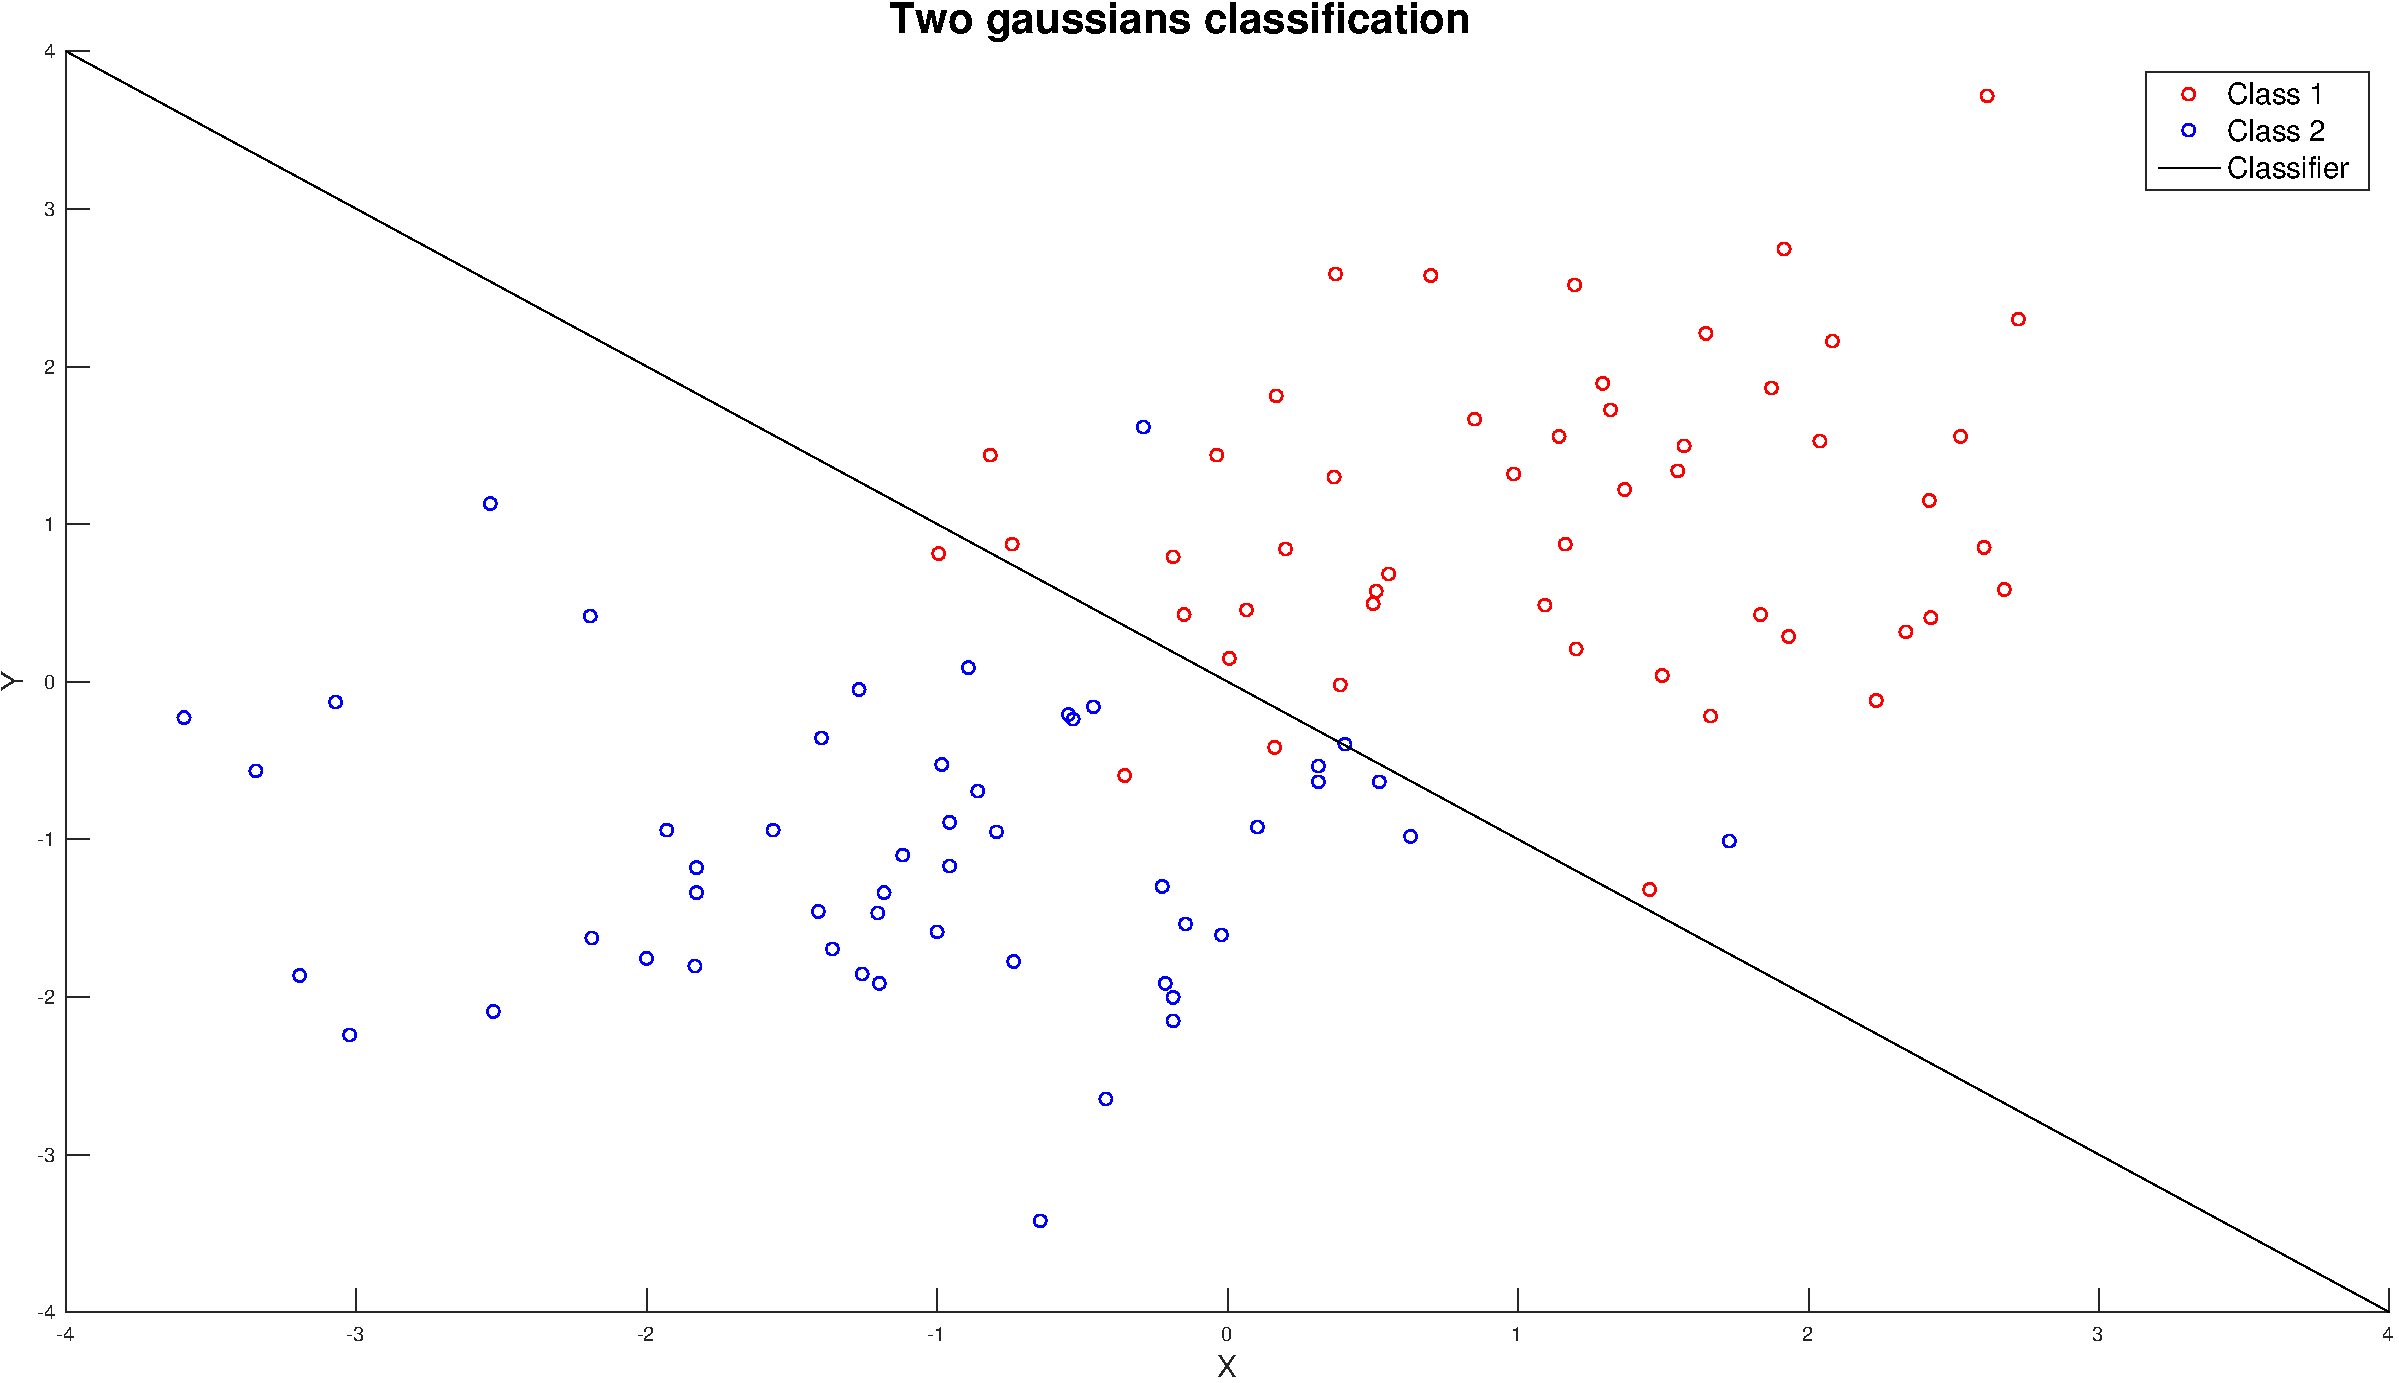
\includegraphics[scale=.40]{two_gaussians.pdf}
    %\caption{Two gaussians classification}
    \label{fig:two_gaussians}
\end{figure}

\section{Support Vector Machine}

The exercises in this section consisted of exploring the properties of
Support Vector Machines via a web application
\footnote{http://cs.stanford.edu/people/karpathy/svmjs/demo/}

\subsection{Linear kernel (subquestions 1 to 3)}
The data with which we are presented in the application is not
linearly separable. Adjusting to a linear kernel, we see that there
are 5 points of each classes, a total of 6 support vectors, 1 point
(green) that is misclassified, and a couple of points inside the
margin, indicating the need for slacking variables (see
\ref{fig:lin1}). With the addition of 10 new points, depending on
where the points are added, you can preserve the total number of
misclassified points (1 green point - see \ref{fig:lin2}). In general,
points added in the same class region, and close to other of the same
class tend not to affect the classifier too much.

Misclassified points can change the classifier drastically,
potentially switching the regions if one class of points outweighs the
other. If the balance of points between the two classes shifts too
much, the region shown in the application frame can become classified
as being of the over-represented class.

\begin{figure}[H]
  \vspace{20pt}
    \centering
    \begin{subfigure}{.5\textwidth}
      \centering
      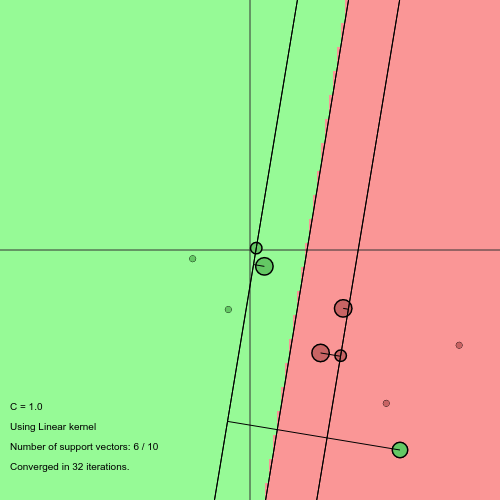
\includegraphics[width=0.9\linewidth]{1-2-1-linear.png}
      \caption{Initial setting (linear kernel)}
      \label{fig:lin1}
    \end{subfigure}%
    \begin{subfigure}{.5\textwidth}
      \centering
      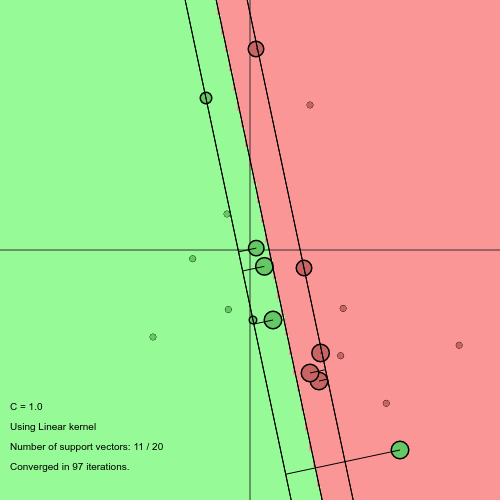
\includegraphics[width=0.9\linewidth]{1-2-1-linear_10.png}
      \caption{After addition of 10 datapoints}
      \label{fig:lin2}
    \end{subfigure}
    \caption{Linear kernel SVM with misclassication}
    \label{fig:bull}
\end{figure}

For the same dataset, varying the values of the hyperparameter for the
regularization impacts the margins of the classifier as shown on
figure \ref{fig:lin3} and \ref{fig:lin4}.


The role of the C parameter is to control the balance in the SVM model
between, on one hand the amount of slacking tolerated, and on the other
hand the maximization of the margin. It is akin to a regularization
hyperparameter, common in statistics (such as ridge regression). In
short, a high value of C results in a smaller tolerance for datapoints
on the wrong side of the margin and results in a margin with a small
width, while a smaller value of C results in a larger margin width and
a higher tolerance for datapoints on the wrong side of the margin.

\begin{figure}[H]
    \centering
    \begin{subfigure}{.5\textwidth}
      \centering
      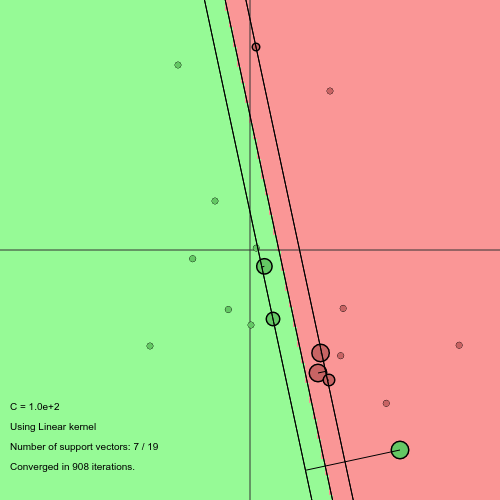
\includegraphics[width=0.9\linewidth]{1-2-1-linear_c_max.png}
      \caption{Value of C: 100}
      \label{fig:lin3}
    \end{subfigure}%
    \begin{subfigure}{.5\textwidth}
      \centering
      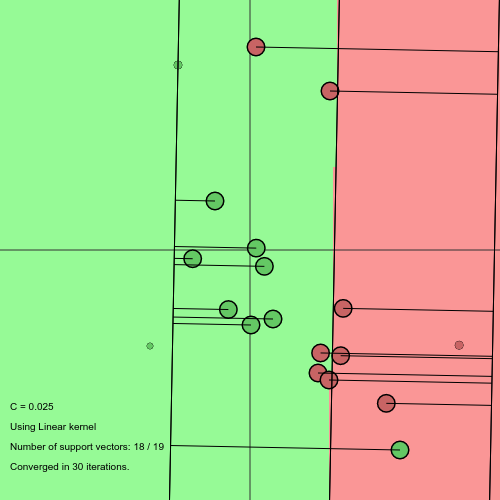
\includegraphics[width=0.9\linewidth]{1-2-1-linear_c_min.png}
      \caption{Value of C: 0.025}
      \label{fig:lin4}
    \end{subfigure}
    \caption{Impact of regularization on the linear classifier boundaries}
    \label{fig:bull}
\end{figure}

\subsection{RBF kernel (subquestions 4 and 5)}

\begin{figure}[H]
    \centering
    \begin{subfigure}[b]{.5\textwidth}
      In this section, we were asked to switch away from a linear kernel and
      opt for the Radial Basis Function kernel (RBF). RBF are localized
      function, centered at a particular value, and use a gaussian fit with
      a certain spread around the center. 

      The same dataset as defined above can be seen on the graphics on
      the right. Here, one can observe that all points have been
      correctly classified, but the area defined are very wobbly,
      displaying clear signs of overfitting.  

      This can be tuned by changing the value of $\sigma$, which
      controls the bandwidth of the gaussian function, see figure
      \ref{fig:RBF_sigma}. Larger values of $\sigma$ leading to more
      linear decision boundaries.
    \end{subfigure}%
    \begin{subfigure}{.5\textwidth}
      \vspace{-185pt}
      \centering
      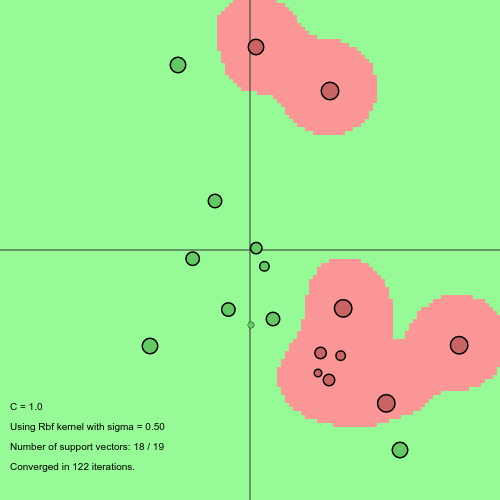
\includegraphics[width=0.9\linewidth]{1-2-1-kernel.png}
      %\caption{RBF kernel}
      %\label{fig:RBF_kernel}
    \end{subfigure}
\end{figure}

\begin{figure}[H]
    \centering
    \begin{subfigure}{.25\textwidth}
      \centering
      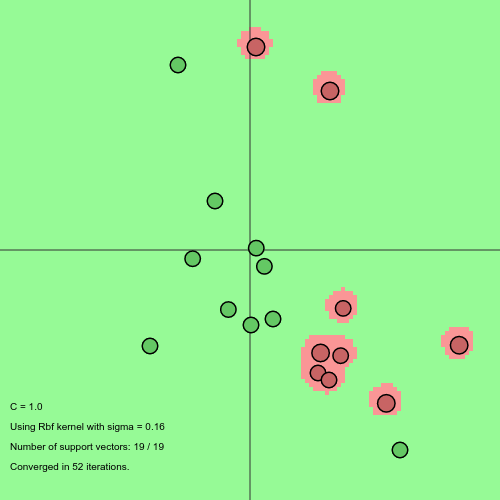
\includegraphics[width=0.9\linewidth]{1-2-1-kernel_ssigma.png}
      \caption{Value of $\sigma = 0.16$}
      \label{fig:rbfs1}
    \end{subfigure}%
    \begin{subfigure}{.25\textwidth}
      \centering
      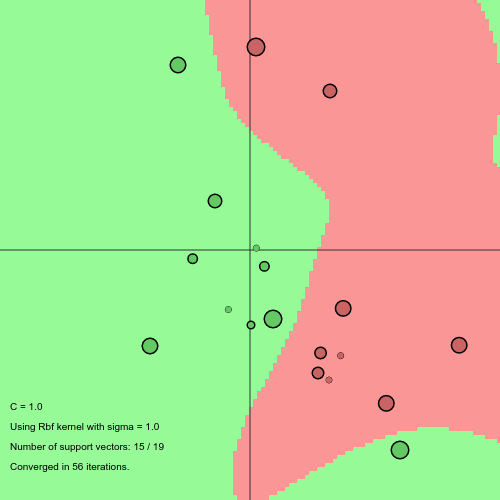
\includegraphics[width=0.9\linewidth]{1-2-1-kernel_ssigma1.png}
      \caption{Value of $\sigma = 1$}
      \label{fig:rbfs2}
    \end{subfigure}%
    \begin{subfigure}{.25\textwidth}
      \centering
      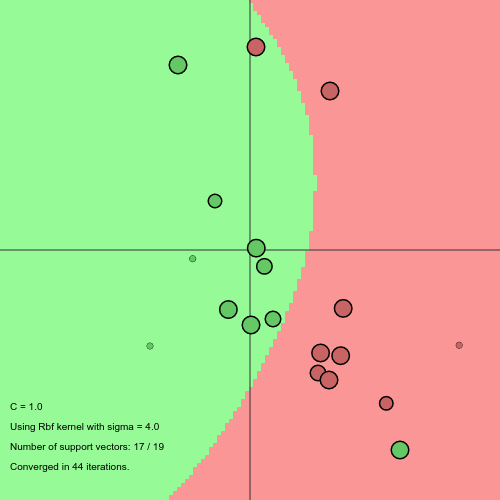
\includegraphics[width=0.9\linewidth]{1-2-1-kernel_ssigma4.png}
      \caption{Value of $\sigma = 4$}
      \label{fig:rbfs3}
    \end{subfigure}%
    \begin{subfigure}{.25\textwidth}
      \centering
      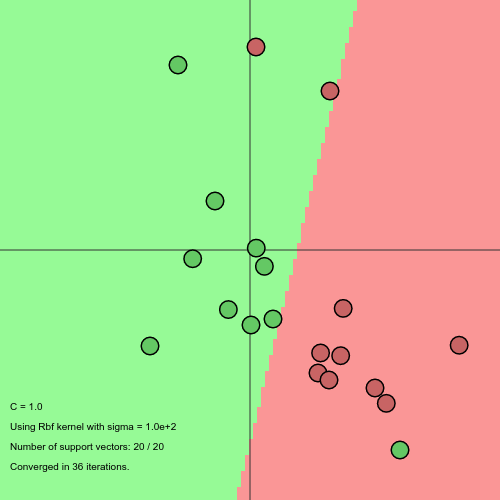
\includegraphics[width=0.9\linewidth]{1-2-1-kernel_ssigma100.png}
      \caption{Value of $\sigma = 100$}
      \label{fig:rfbs4}
    \end{subfigure}
    \caption{Impact of $\sigma$ on the RBF classifier boundaries (C=1.0)}
    \label{fig:RBF_sigma}
\end{figure}

From the experimentation with the application, I would tend to think
that in the case of an almost linearly separable dataset, a large
value for $\sigma$ is preferable, with a value for C of 1.0 (possibly
optimized depending on the amount of misclassified points).

\subsection{Kernel (subquestion 6)}

For this question, I generated a balanced dataset of points (25 points
for each class, hence 50 points in total), with the goal in mind of
having a linear classifier work best. I was able to obtain a good
definition of the decision surface using both the linear kernel, but
also the RBF kernel after some tuning. However, the linear kernel was
straightforward to use, as the C parameter did not have much impact
except for extreme values. The minimum number of support vectors
achievable in both cases was also similar. 

\begin{figure}[H]
    \centering
    \begin{subfigure}{.5\textwidth}
      \centering
      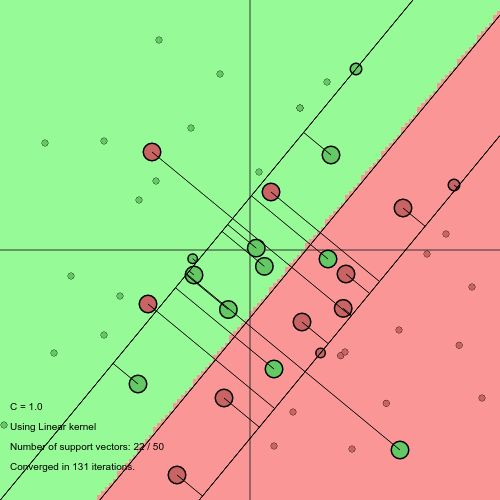
\includegraphics[width=0.9\linewidth]{1-2-1-kernel6n2.png}
      \caption{Linear classifier}
      \label{fig:rbf_linclass}
    \end{subfigure}%
    \begin{subfigure}{.5\textwidth}
      \centering
      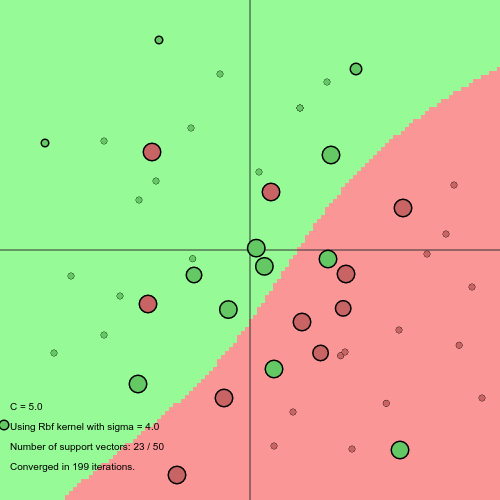
\includegraphics[width=0.9\linewidth]{1-2-1-kernel6n.png}
      \caption{RBF kernel classifier}
      \label{fig:rbf_class}
    \end{subfigure}
    \caption{Classification using linear SVM and RBF kernel SVM}
    \label{fig:rbf_lin_data}
\end{figure}

\subsection{Support vectors (subquestion 7 and 8)}

Support vectors are vectors in the data space (p-dimensional) that
support the maximal margin hyperplane (in the feature space using the
kernel trick for the RBF). If those particular vectors are moved, then
the resulting margin moves as well. Importantly, the classifier's
decision boundary depends only on these support vectors, hence the
classifier can be expressed using them. This can result in an
advantage in terms of compression, as the dataset can be trimmed down
after training, saving only those support vectors that are necessary
for the classifier.

In the figure \ref{fig:ker7reduced} below, one can see such an effect
of compression. Originally, 150 datapoints were present, but only 10
of them are necessary to construct a satisfying classifier. In this
example, I played around with the parameters to obtain the reduced
number of support vectors. In figure \ref{fig:ker7spiral} however, the
entire dataset (highly non-linear) consists of the support vectors. It
is not possible to reduce the amount of support vectors by tuning the
parameters without impacting with much detriment the boundaries of the
classifier.

A datapoint becomes a support vector when it is in proximity of the
margin of the classifer, or if it is misclassified. From the
experimentation on the web application, we can see that anytime a
point is added in the wrong region, or within the margin, it becomes a
support vector.

\begin{figure}[H]
    \centering
    \begin{subfigure}{.5\textwidth}
      \centering
      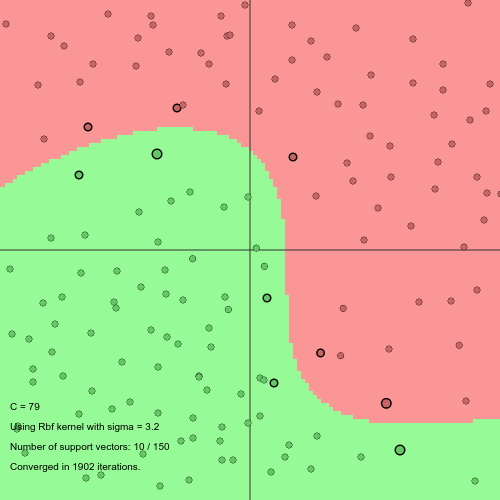
\includegraphics[width=0.9\linewidth]{1-2-1-kernel7.png}
      \caption{Few support vectors needed (10/150)}
      \label{fig:ker7reduced}
    \end{subfigure}%
    \begin{subfigure}{.5\textwidth}
      \centering
      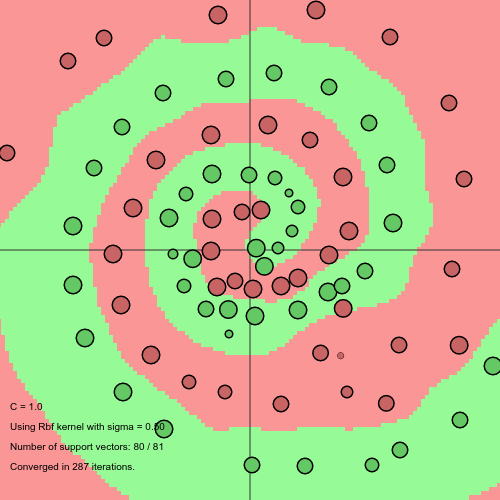
\includegraphics[width=0.9\linewidth]{1-2-1-kernel7spiral.png}
      \caption{No compression}
      \label{fig:ker7spiral}
    \end{subfigure}
    \caption{Support vectors}
    \label{fig:ker7}
\end{figure}

\section{Least-Squares Support Vector Machine}

\subsection{Iris dataset}

\subsubsection{LS-SVM sample script exploration}
For this section, I explored the iris dataset using the LS-SVM library
developed at KU Leuven. The dataset contains 2 distinct classes that
are not linearly separable.

The figure \ref{fig:iris_linpol} below summarizes visually the
classifiers built using linear and polynomial kernels for the
classification task. For the polynomial kernel, I used degree 2, 3,
and 4. When using a polynomial of degree 1, I obviously get exactly
the same results as when using a linear kernel. In the table
\ref{table:iris_linpol}, you can see the error rate on the test set
dropping as the flexibility of our model is raised. The very wobbly
region defined by the kernel of degree 4 seem to display signs of
overfitting as the region in the top-rigth corner. Overfitting
typically leads to poor generalization.

Since the dataset consists of regions that are not linearly separable,
the linear kernel performs terribly. It is not obvious to me that there
is a connection between the $\sigma^2$ parameter of the RBF kernel,
which controls the spread around the center in the gaussian, and the
degree of the polynomial kernel. I would expect that overfitting would
occur in tandem as you lower the value of $sigma^2$, and increase the
degree of the polynomial.

\begin{table}[H]
  \centering
  \begin{tabular}{l|l|l|}
    \cline{2-3}
    & \# Missclassified & \% Error \\ \hline
    \multicolumn{1}{|l|}{Linear kernel}       & 11                & 55\%     \\ \hline
    \multicolumn{1}{|l|}{Polynomial degree 2} & 5                 & 5\%      \\ \hline
    \multicolumn{1}{|l|}{Polynomial degree 3} & 0                 & 0\%      \\ \hline
    \multicolumn{1}{|l|}{Polynomial degree 4} & 0                 & 0\%      \\ \hline
  \end{tabular}
  \caption{Missclassification summary (polynomial kernel)}
  \label{table:iris_linpol}
\end{table}

\begin{figure}[H]
    \centering
    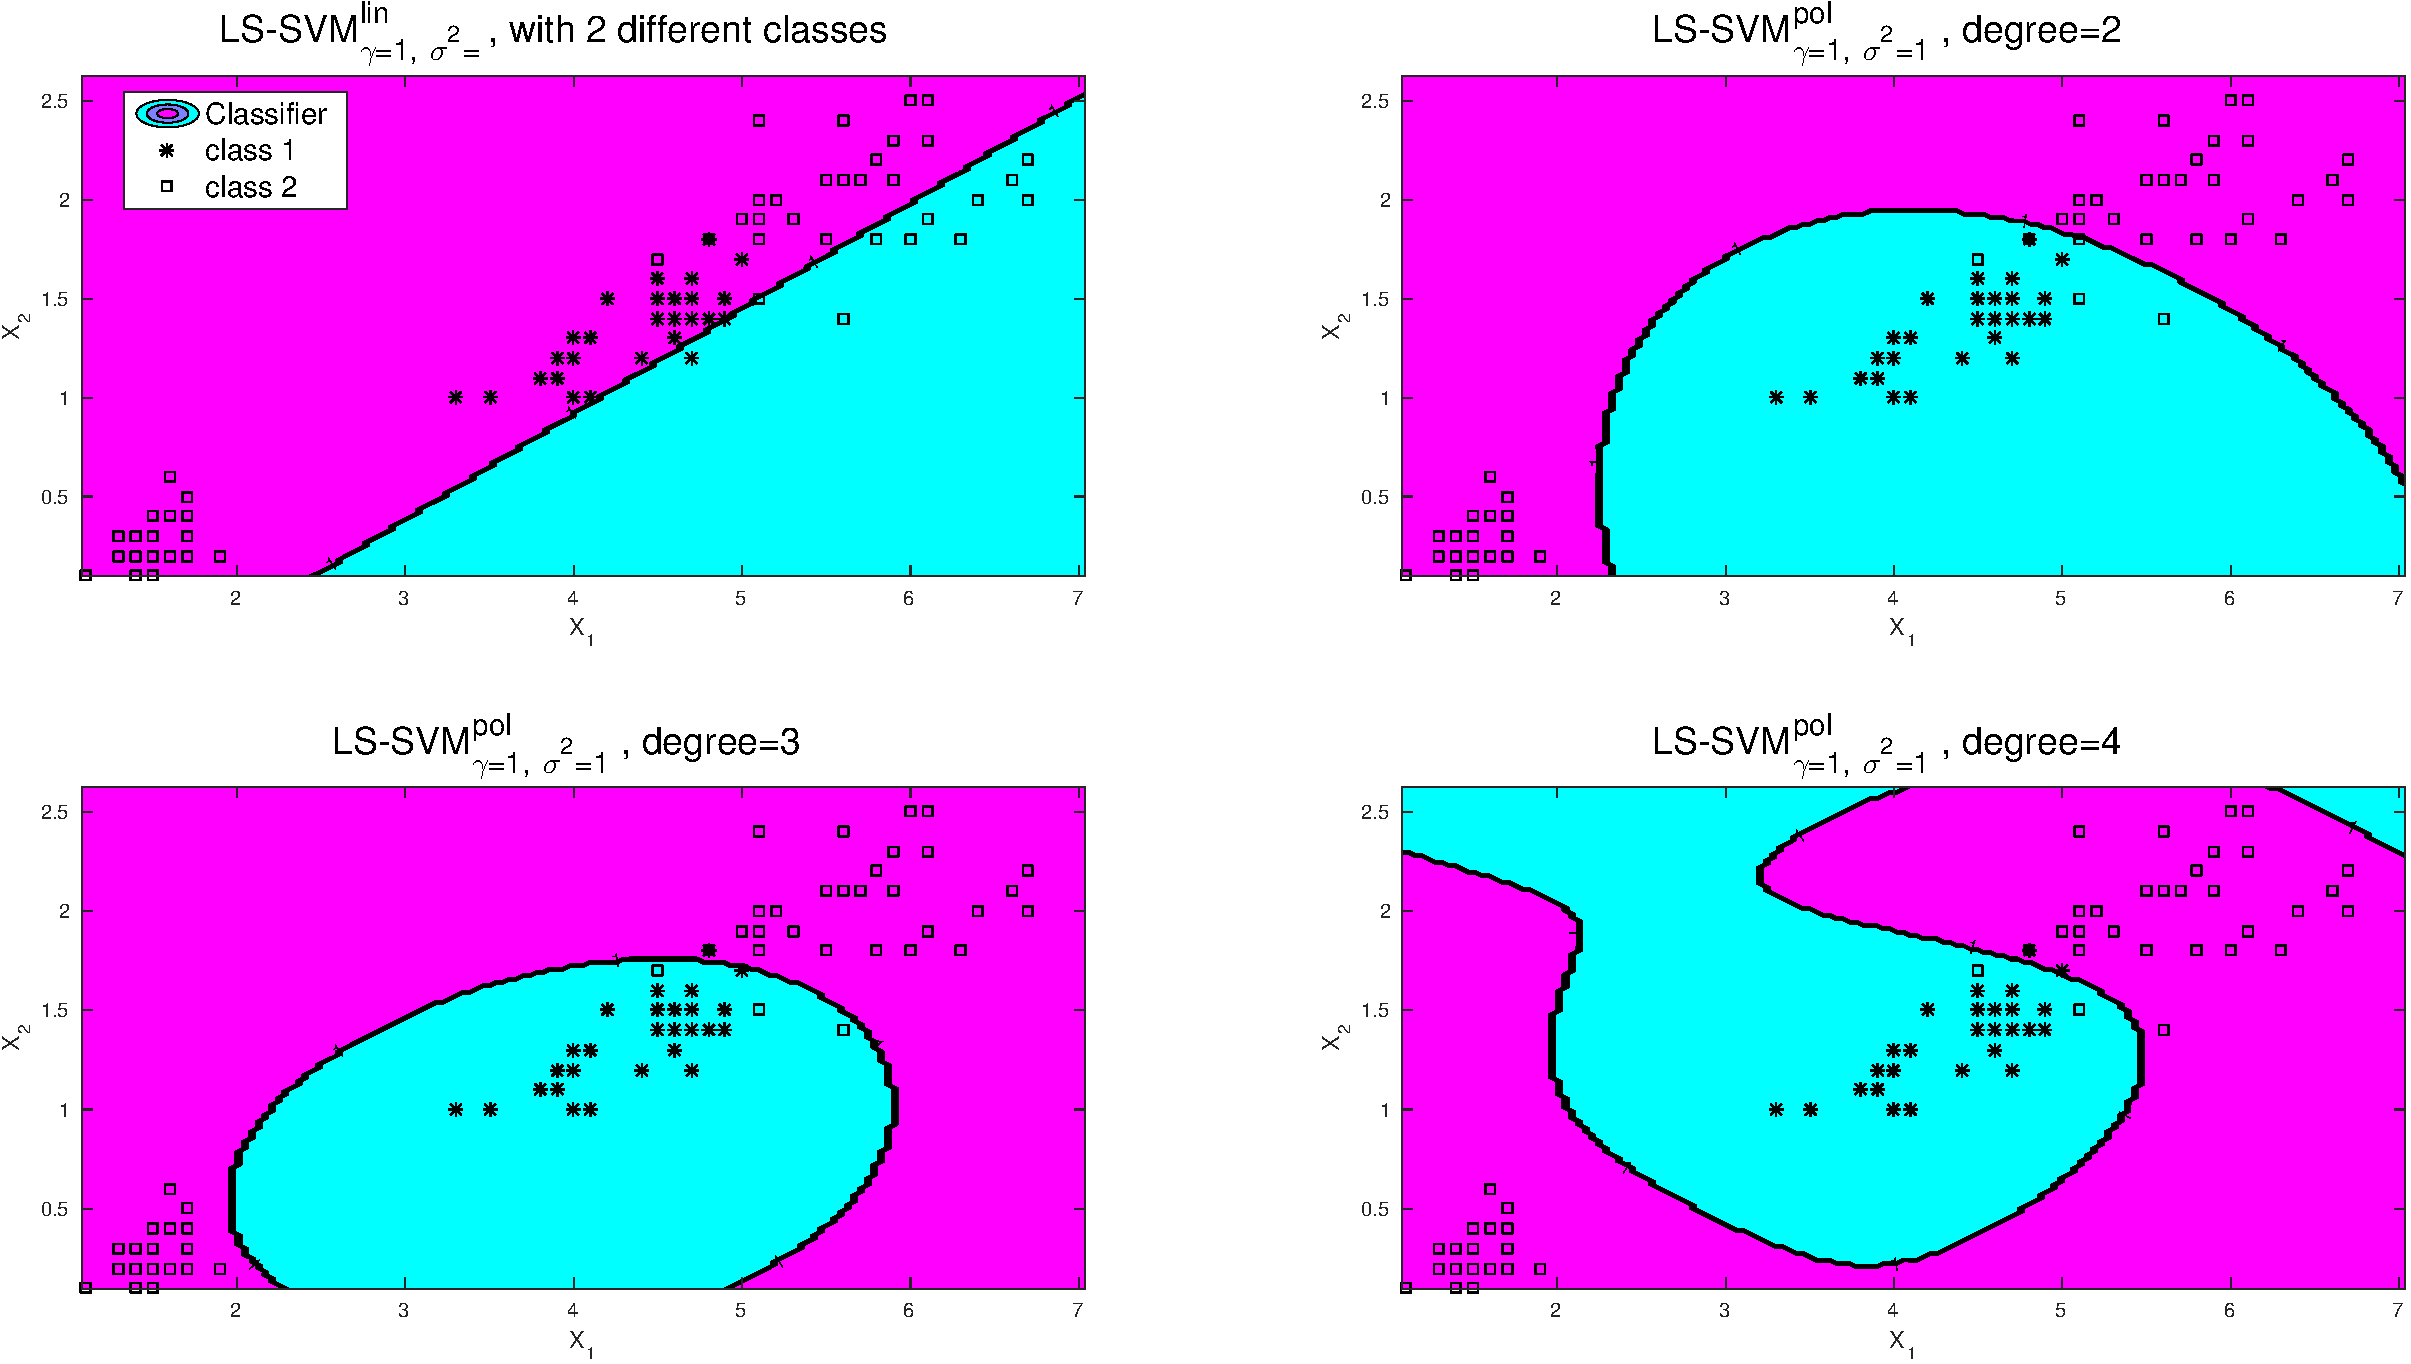
\includegraphics[scale=.40]{iris_linpol.pdf}
    \caption{Linear and polynomial kernel classifiers}
    \label{fig:iris_linpol}
\end{figure}


\begin{figure}[H]
    \centering
    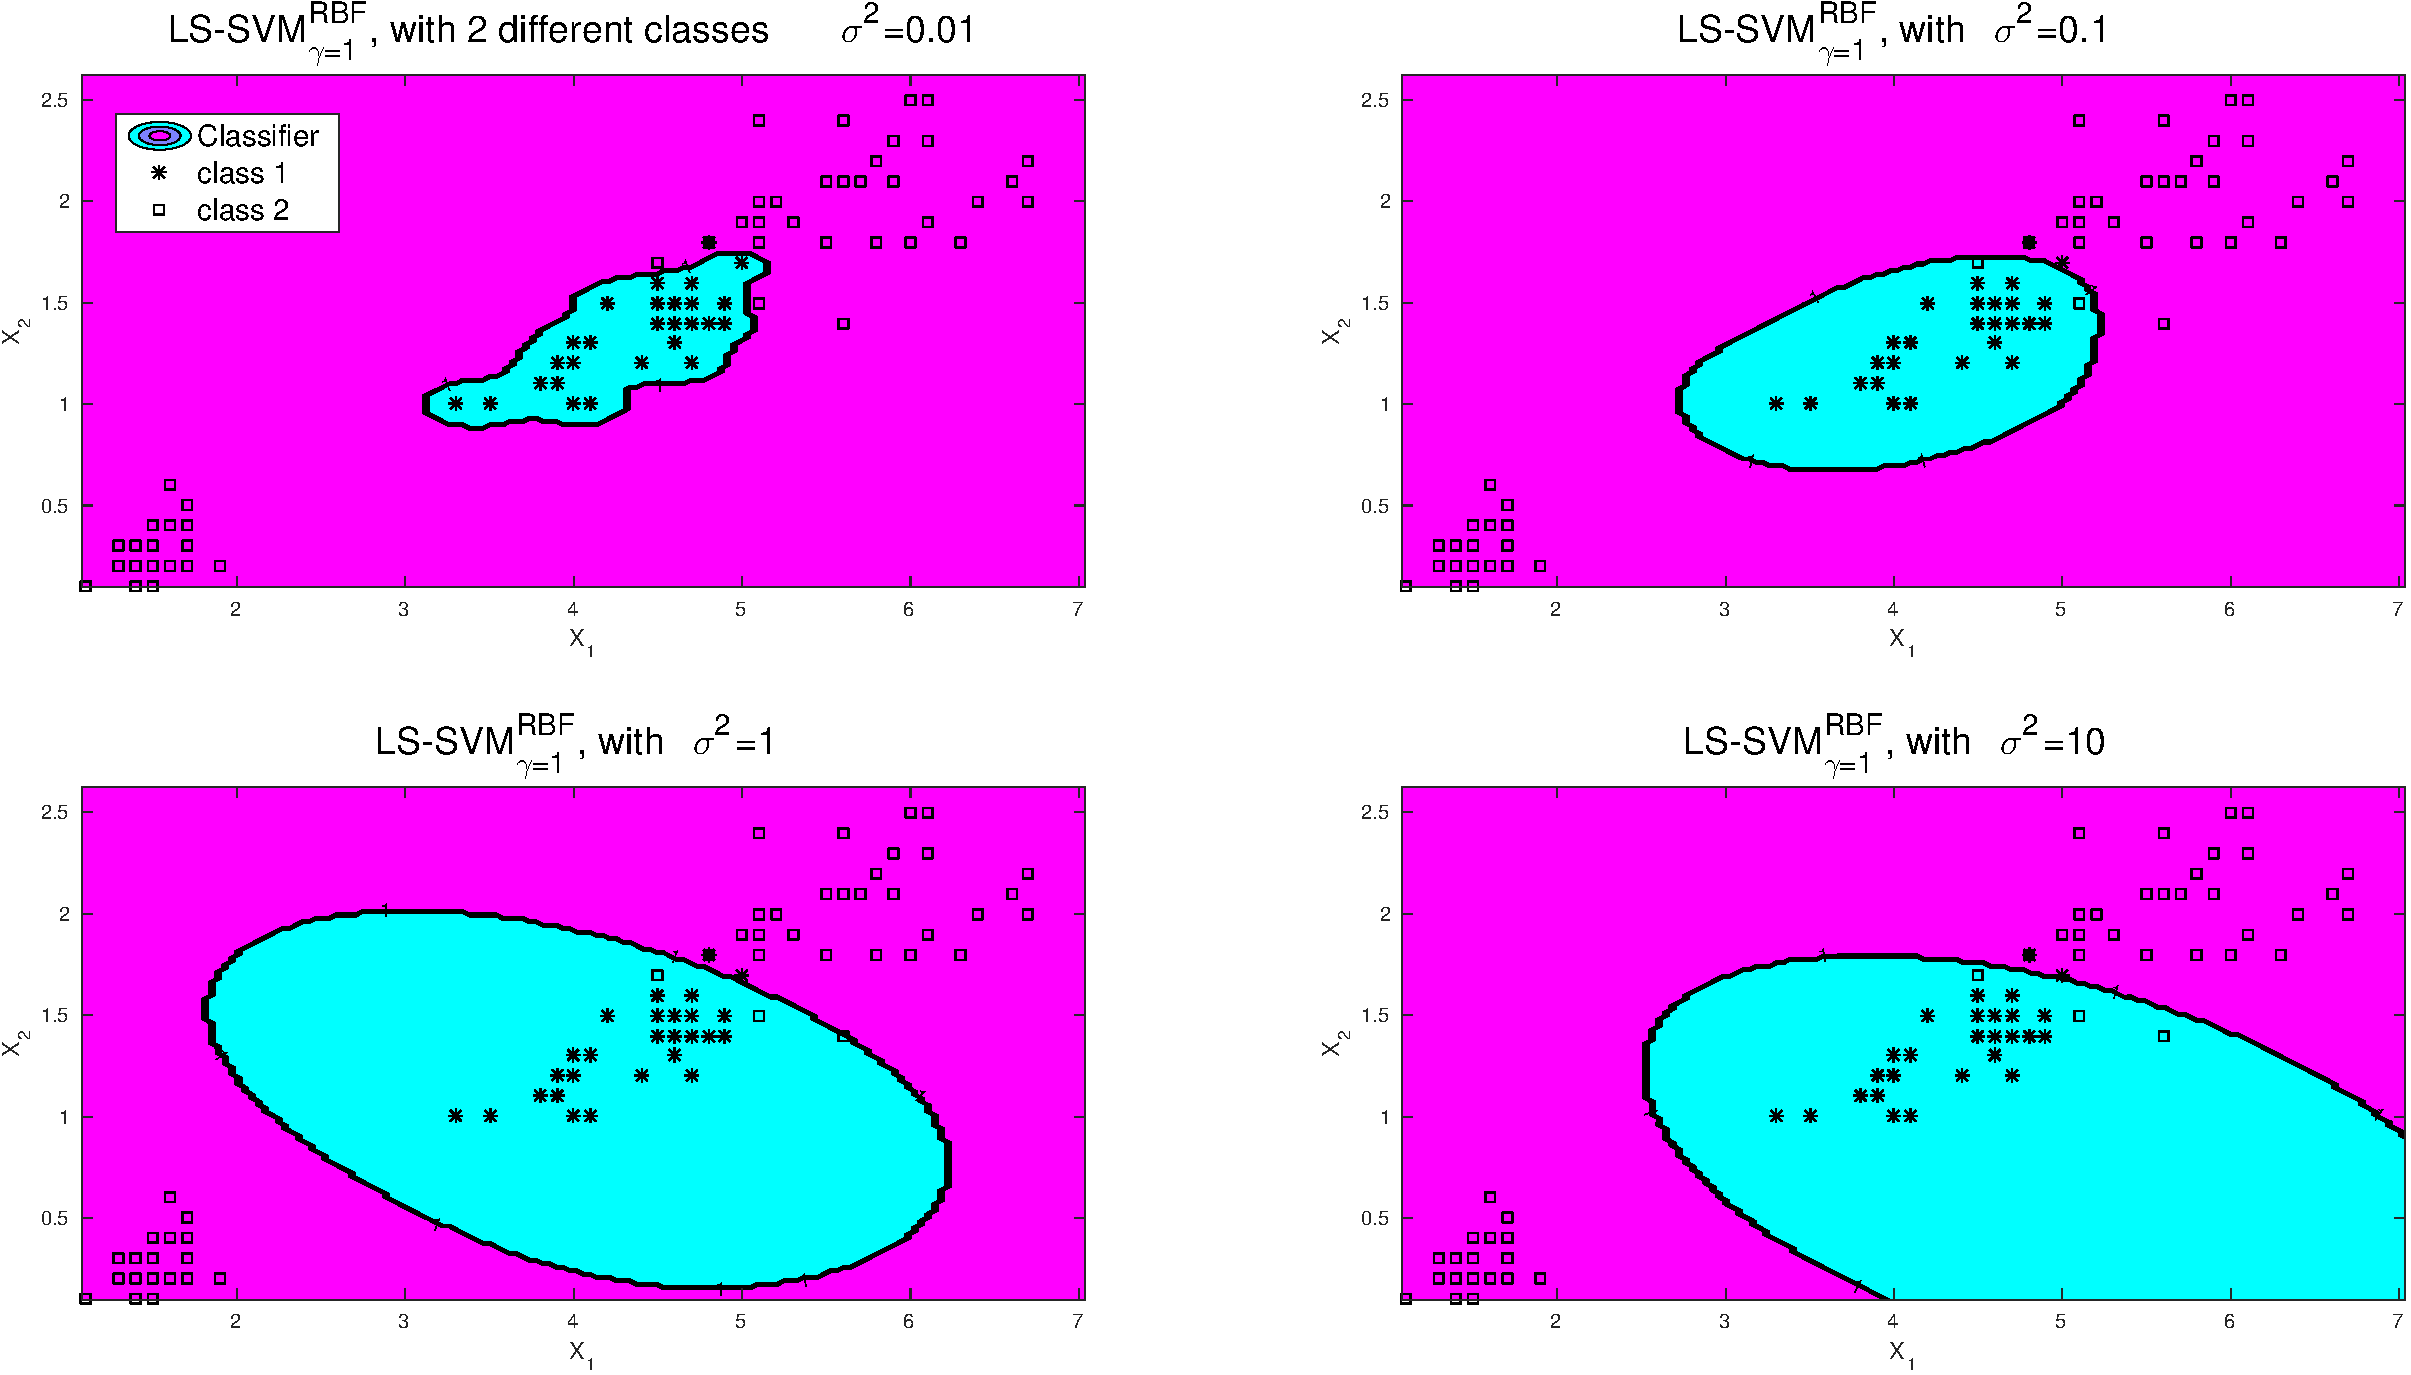
\includegraphics[scale=.40]{iris_rbf.pdf}
    \caption{RBF classifier with different values of sigma}
    \label{fig:iris_linpol}
\end{figure}

\begin{table}[]
  \centering
  \begin{tabular}{l|l|l|}
    \cline{2-3}
    & \# Misclassified & \% Error \\ \hline
    \multicolumn{1}{|l|}{RBF $\gamma=1$, $\sigma^2=0.01$} & 2                 & 10\%     \\ \hline
    \multicolumn{1}{|l|}{RBF $\gamma=1$, $\sigma^2=0.1$}  & 0                 & 0\%      \\ \hline
    \multicolumn{1}{|l|}{RBF $\gamma=1$, $\sigma^2=1$}    & 0                 & 0\%      \\ \hline
    \multicolumn{1}{|l|}{RBF $\gamma=1$, $\sigma^2=10$}   & 0                 & 0\%      \\ \hline
  \end{tabular}
  \label{table:iris_rbf}
  \caption{Misclassification summary (RBF kernel)}
\end{table}

This last figure \ref{fig:iris_overfitting} illustrate a bit one of
the extremes of the bias-variance tradeoff and overfitting. As seen in
the previous graphs, with less flexible models, and especially in this
case with a linear model (high bias), you run the risk of not
capturing the pattern in your dataset correctly and get terrible
results on the test set. On the other end of the spectrum, with very
flexible models, your variance increases too much and although the
performance on the training set are close to perfection, the results
on the test set are off (see table 3). Typically, you have
\emph{memorized} your dataset, but failed to obtain good
generalization.

\begin{table}[H]
  \centering
  \begin{tabular}{l|l|l|}
    \cline{2-3}
    & \# Misclassified & \% Error \\ \hline
    \multicolumn{1}{|l|}{RBF $\gamma=1$, $\sigma^2=0.001$} & 6                 & 30\%     \\ \hline
    \multicolumn{1}{|l|}{RBF $\gamma=1$, $\sigma^2=0.01$}  & 2                 & 10\%      \\ \hline
    \multicolumn{1}{|l|}{Polynomial degree 15}    & 1                 & 5\%      \\ \hline
    \multicolumn{1}{|l|}{Polynomial degree 20}   & 4                 & 20\%      \\ \hline
  \end{tabular}
  \label{table:iris_over}
  \caption{Misclassification summary (Overfitting)}
\end{table}

\begin{figure}[H]
    \centering
    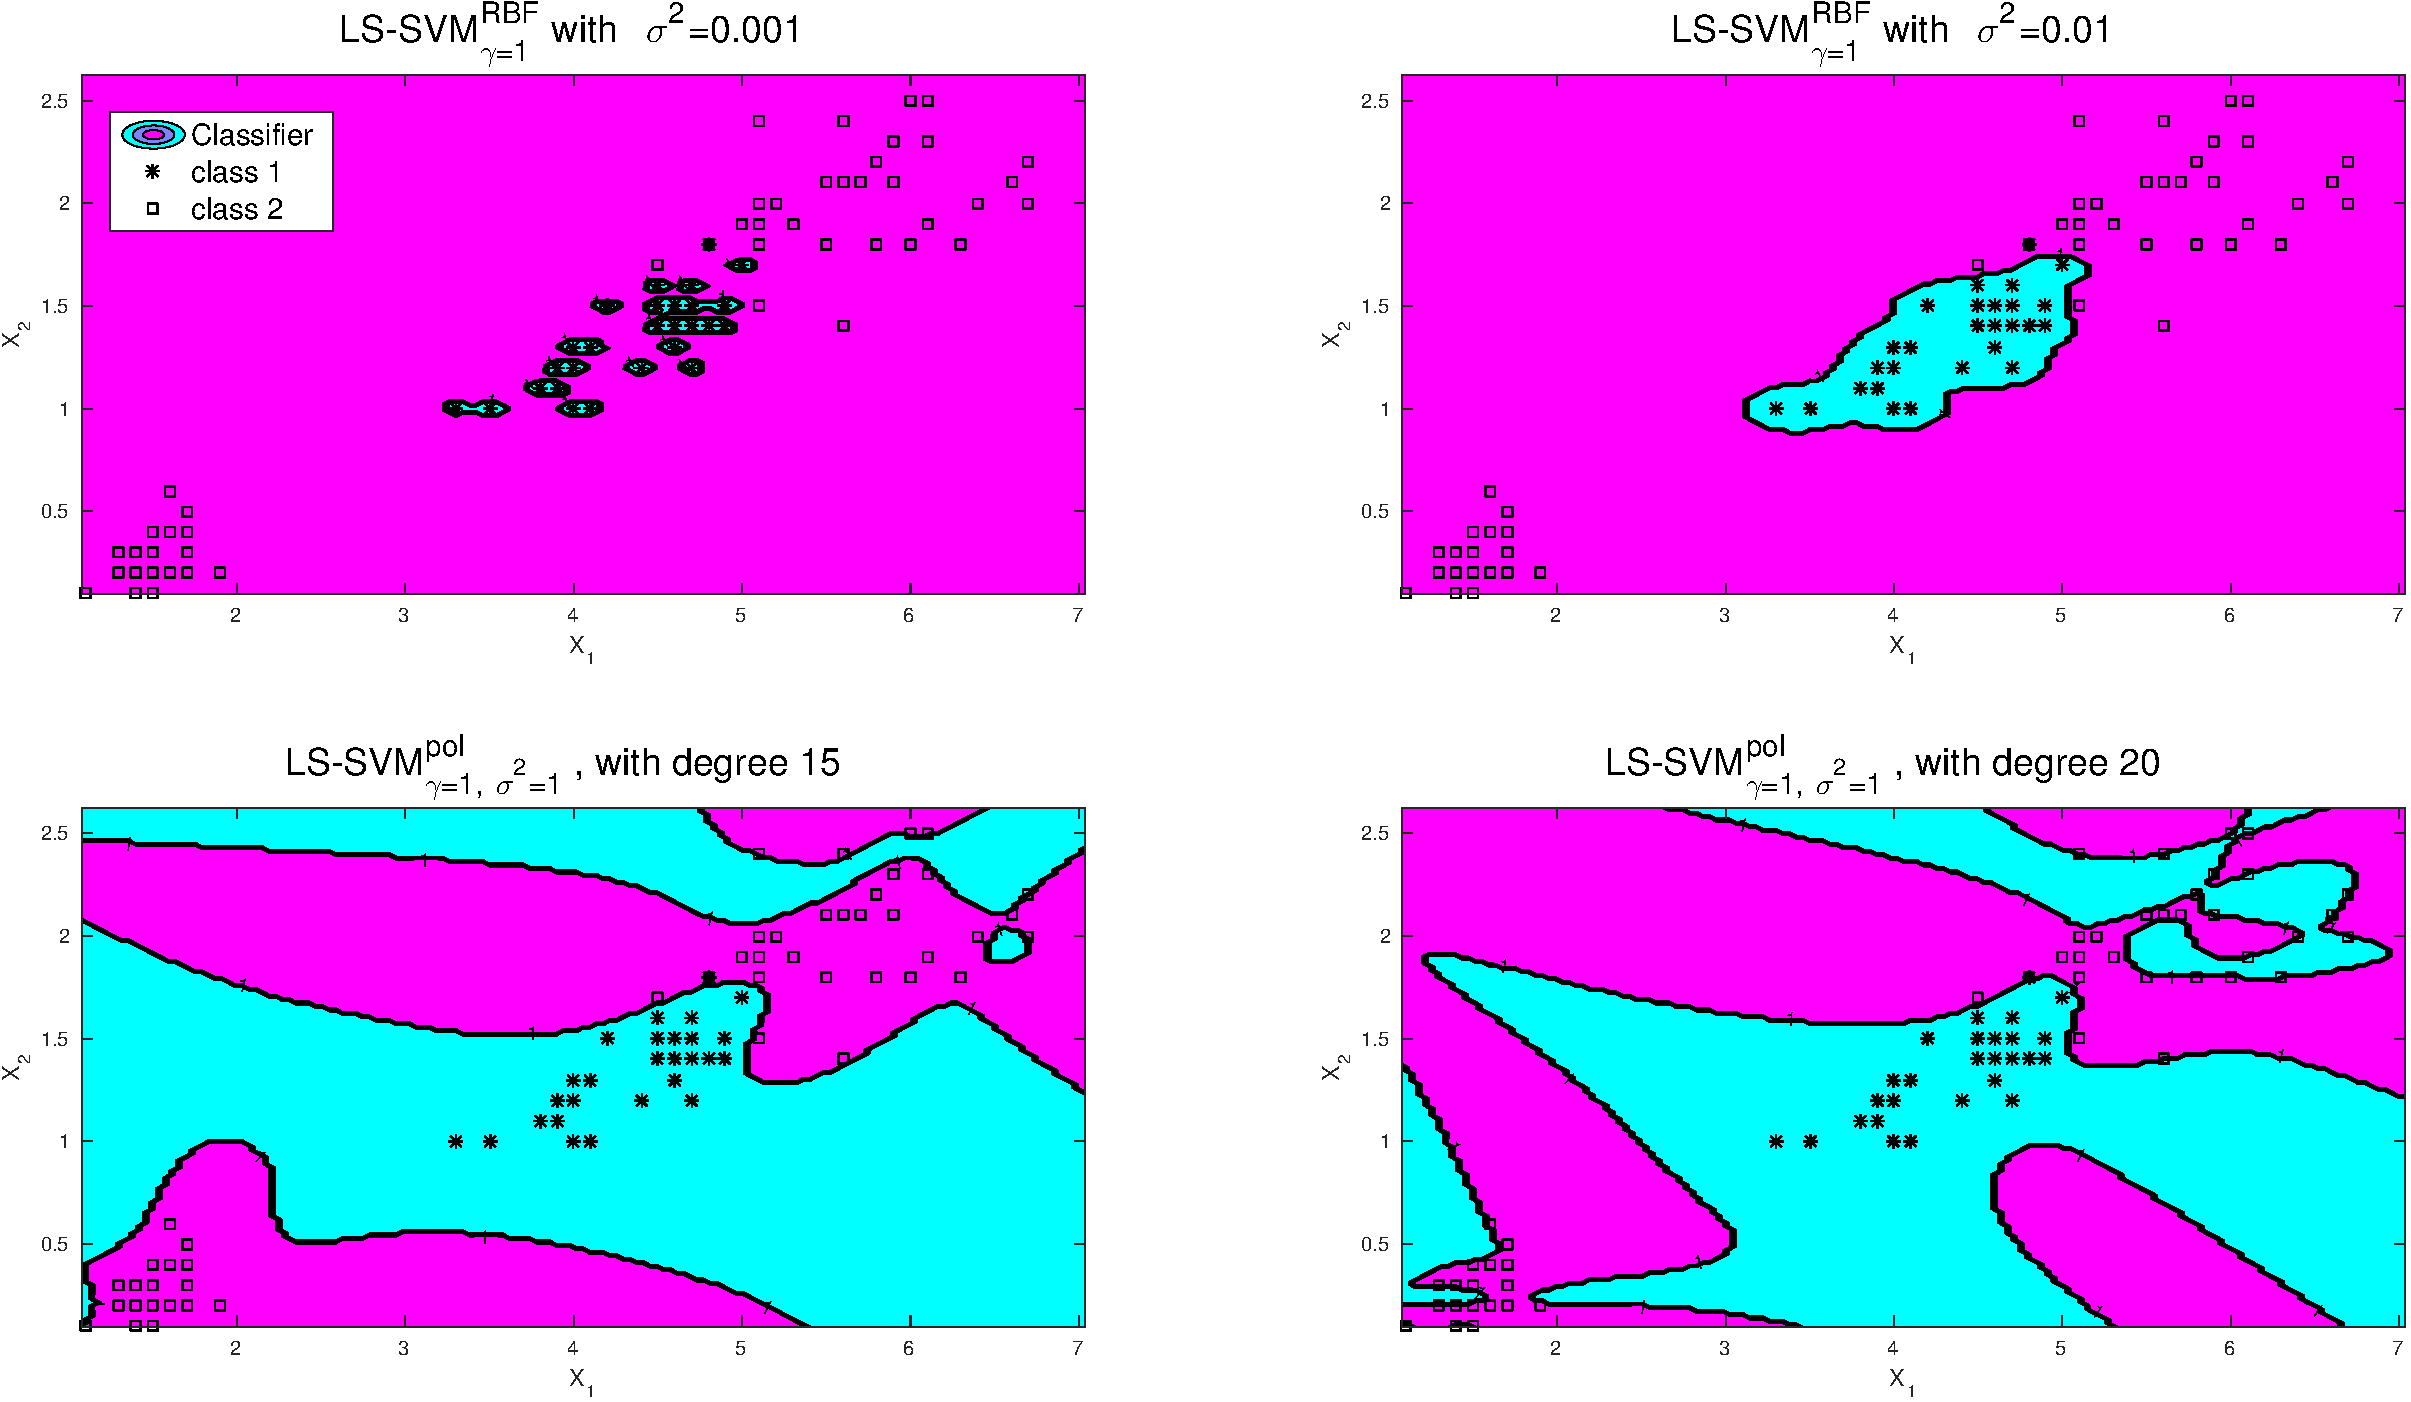
\includegraphics[scale=.40]{iris_overfitting.pdf}
    \caption{Overfitting with polynomial and RBF kernels}
    \label{fig:iris_overfitting}
\end{figure}

\subsubsection{RBF kernel: sigma}

In this section, we explore further the effect of the bandwidth
parameter $\sigma^2$ for the RBF kernel and its effect on
generalization as measured on a test set.

Below is the corresponding matlab code and figure \ref{fig:rbf_sigma}
used to establish the interval out of which to pick a reasonable
$\sigma^2$. The idea here is to fix the value of $\gamma$ to 1, and
establish a logarithmic grid of possible values for $\sigma^2$,
systematically building models using the training set and evaluating
the performance on the test set.

This allows us to define an interval for the choice of the parameter:
$\sigma^2 \in [0.1,10]$

\begin{lstlisting}
gam = 1; type='c'; sig2list=logspace(-3,3,60); errlist=[];

for sig2=sig2list,
    [alpha,b] = trainlssvm({X,Y,type,gam,sig2,'RBF_kernel'});
    % Obtain classification of test set using trained classifier
    [Yht, Zt] = simlssvm({X,Y,type,gam,sig2,'RBF_kernel'}, {alpha,b}, Xt);
    err = sum(Yht~=Yt); errlist = [errlist; err]; 
end

figure('Color',[1 1 1]);
semilogx(sig2list, errlist./20.*100, 'b-');
title('Test missclassification vs. Sigma');
xlabel('Sigma (log_{10})'); ylabel('Missclassification %');
\end{lstlisting}

\begin{figure}[H]
    \centering
    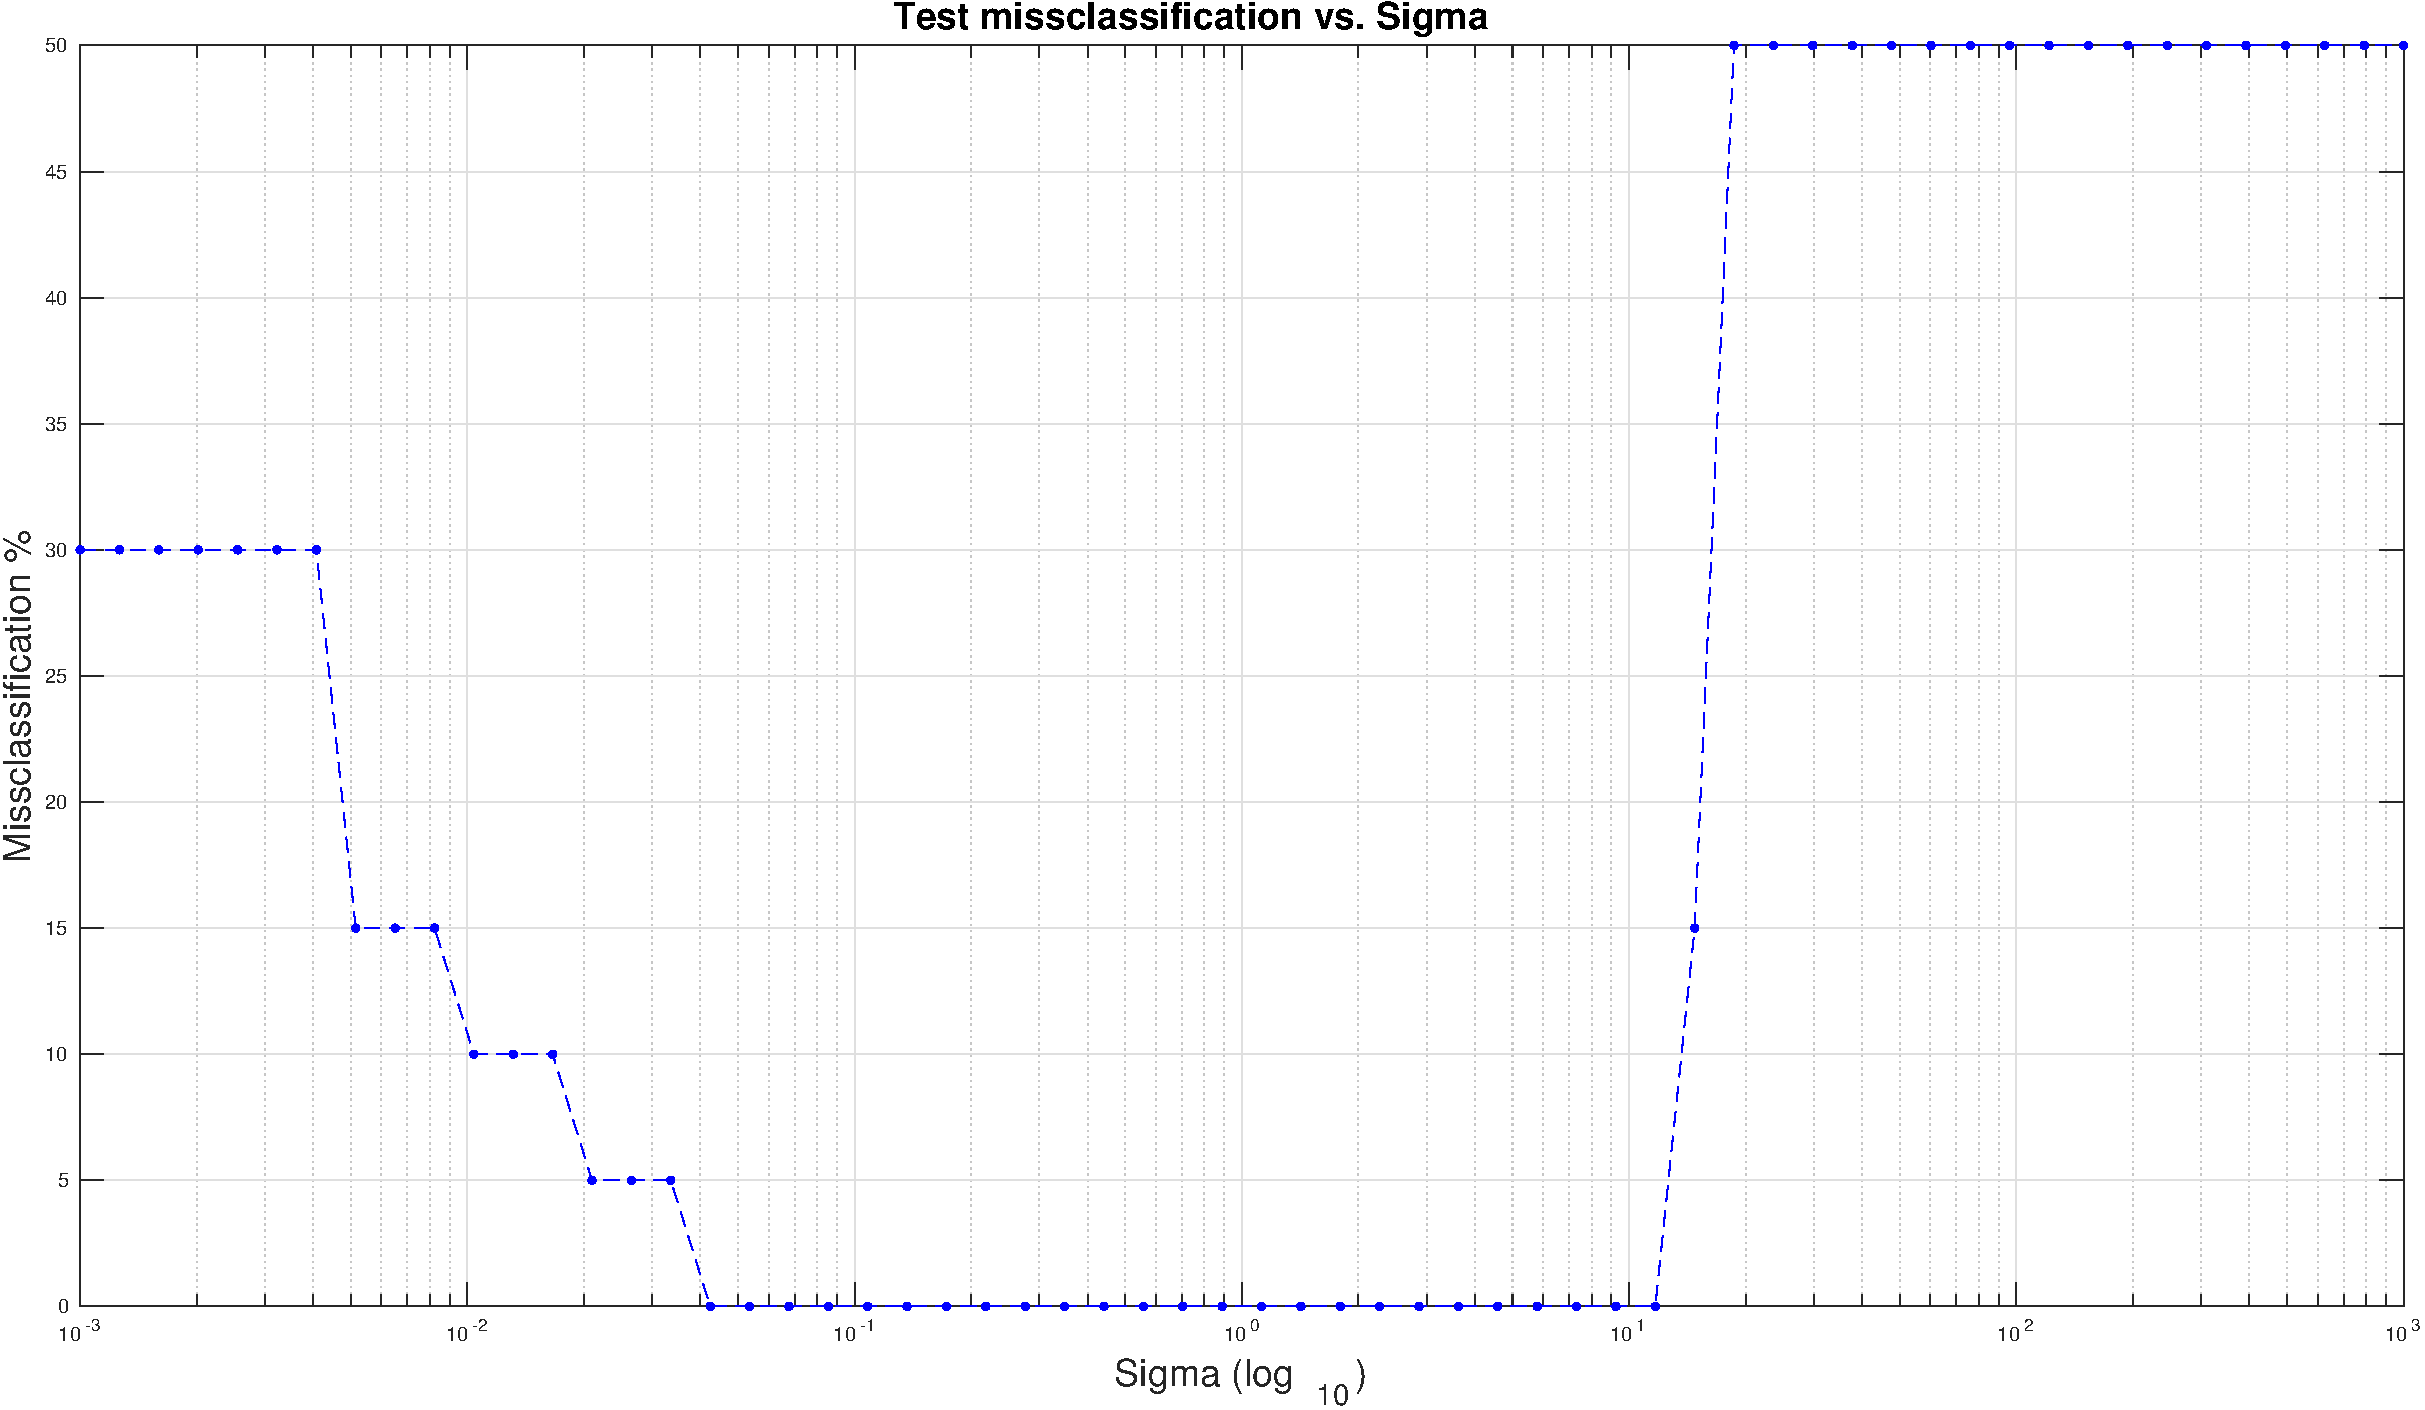
\includegraphics[scale=.40]{rbf_sigma.pdf}
    \caption{Tuning of parameter $\sigma^2$ for fixed $\gamma=1$}
    \label{fig:rbf_sigma}
\end{figure}

\subsubsection{RBF kernel: regularization constant}

In this section, we explore further the effect of the tuning parameter
$\gamma$, used for regularization (to control the amount of slack
variables for non-separable data), and its effect on generalization as
measured on a test set.

The procedure to select the value of the hyperparameter is the same as
described in the previous section. The result indicates to chose
$\gamma \in [0.15,80]$
\begin{lstlisting}
sig2 = 0.1; gamlist=logspace(-3,3,60); type='c'; errlist=[];

for gam=gamlist,
    [alpha,b] = trainlssvm({X,Y,type,gam,sig2,'RBF_kernel'});
    % Obtain classification of test set using trained classifier
    [Yht, Zt] = simlssvm({X,Y,type,gam,sig2,'RBF_kernel'}, {alpha,b}, Xt);
    err = sum(Yht~=Yt); errlist = [errlist; err];
end

figure('Color',[1 1 1]);
semilogx(gamlist, errlist./20.*100, 'b-');
title('Test missclassification vs. Gamma (fixed \sigma^2=0.1)');
xlabel('\gamma (log_{10})'); ylabel('Missclassification %');
\end{lstlisting}

\begin{figure}[H]
    \centering
    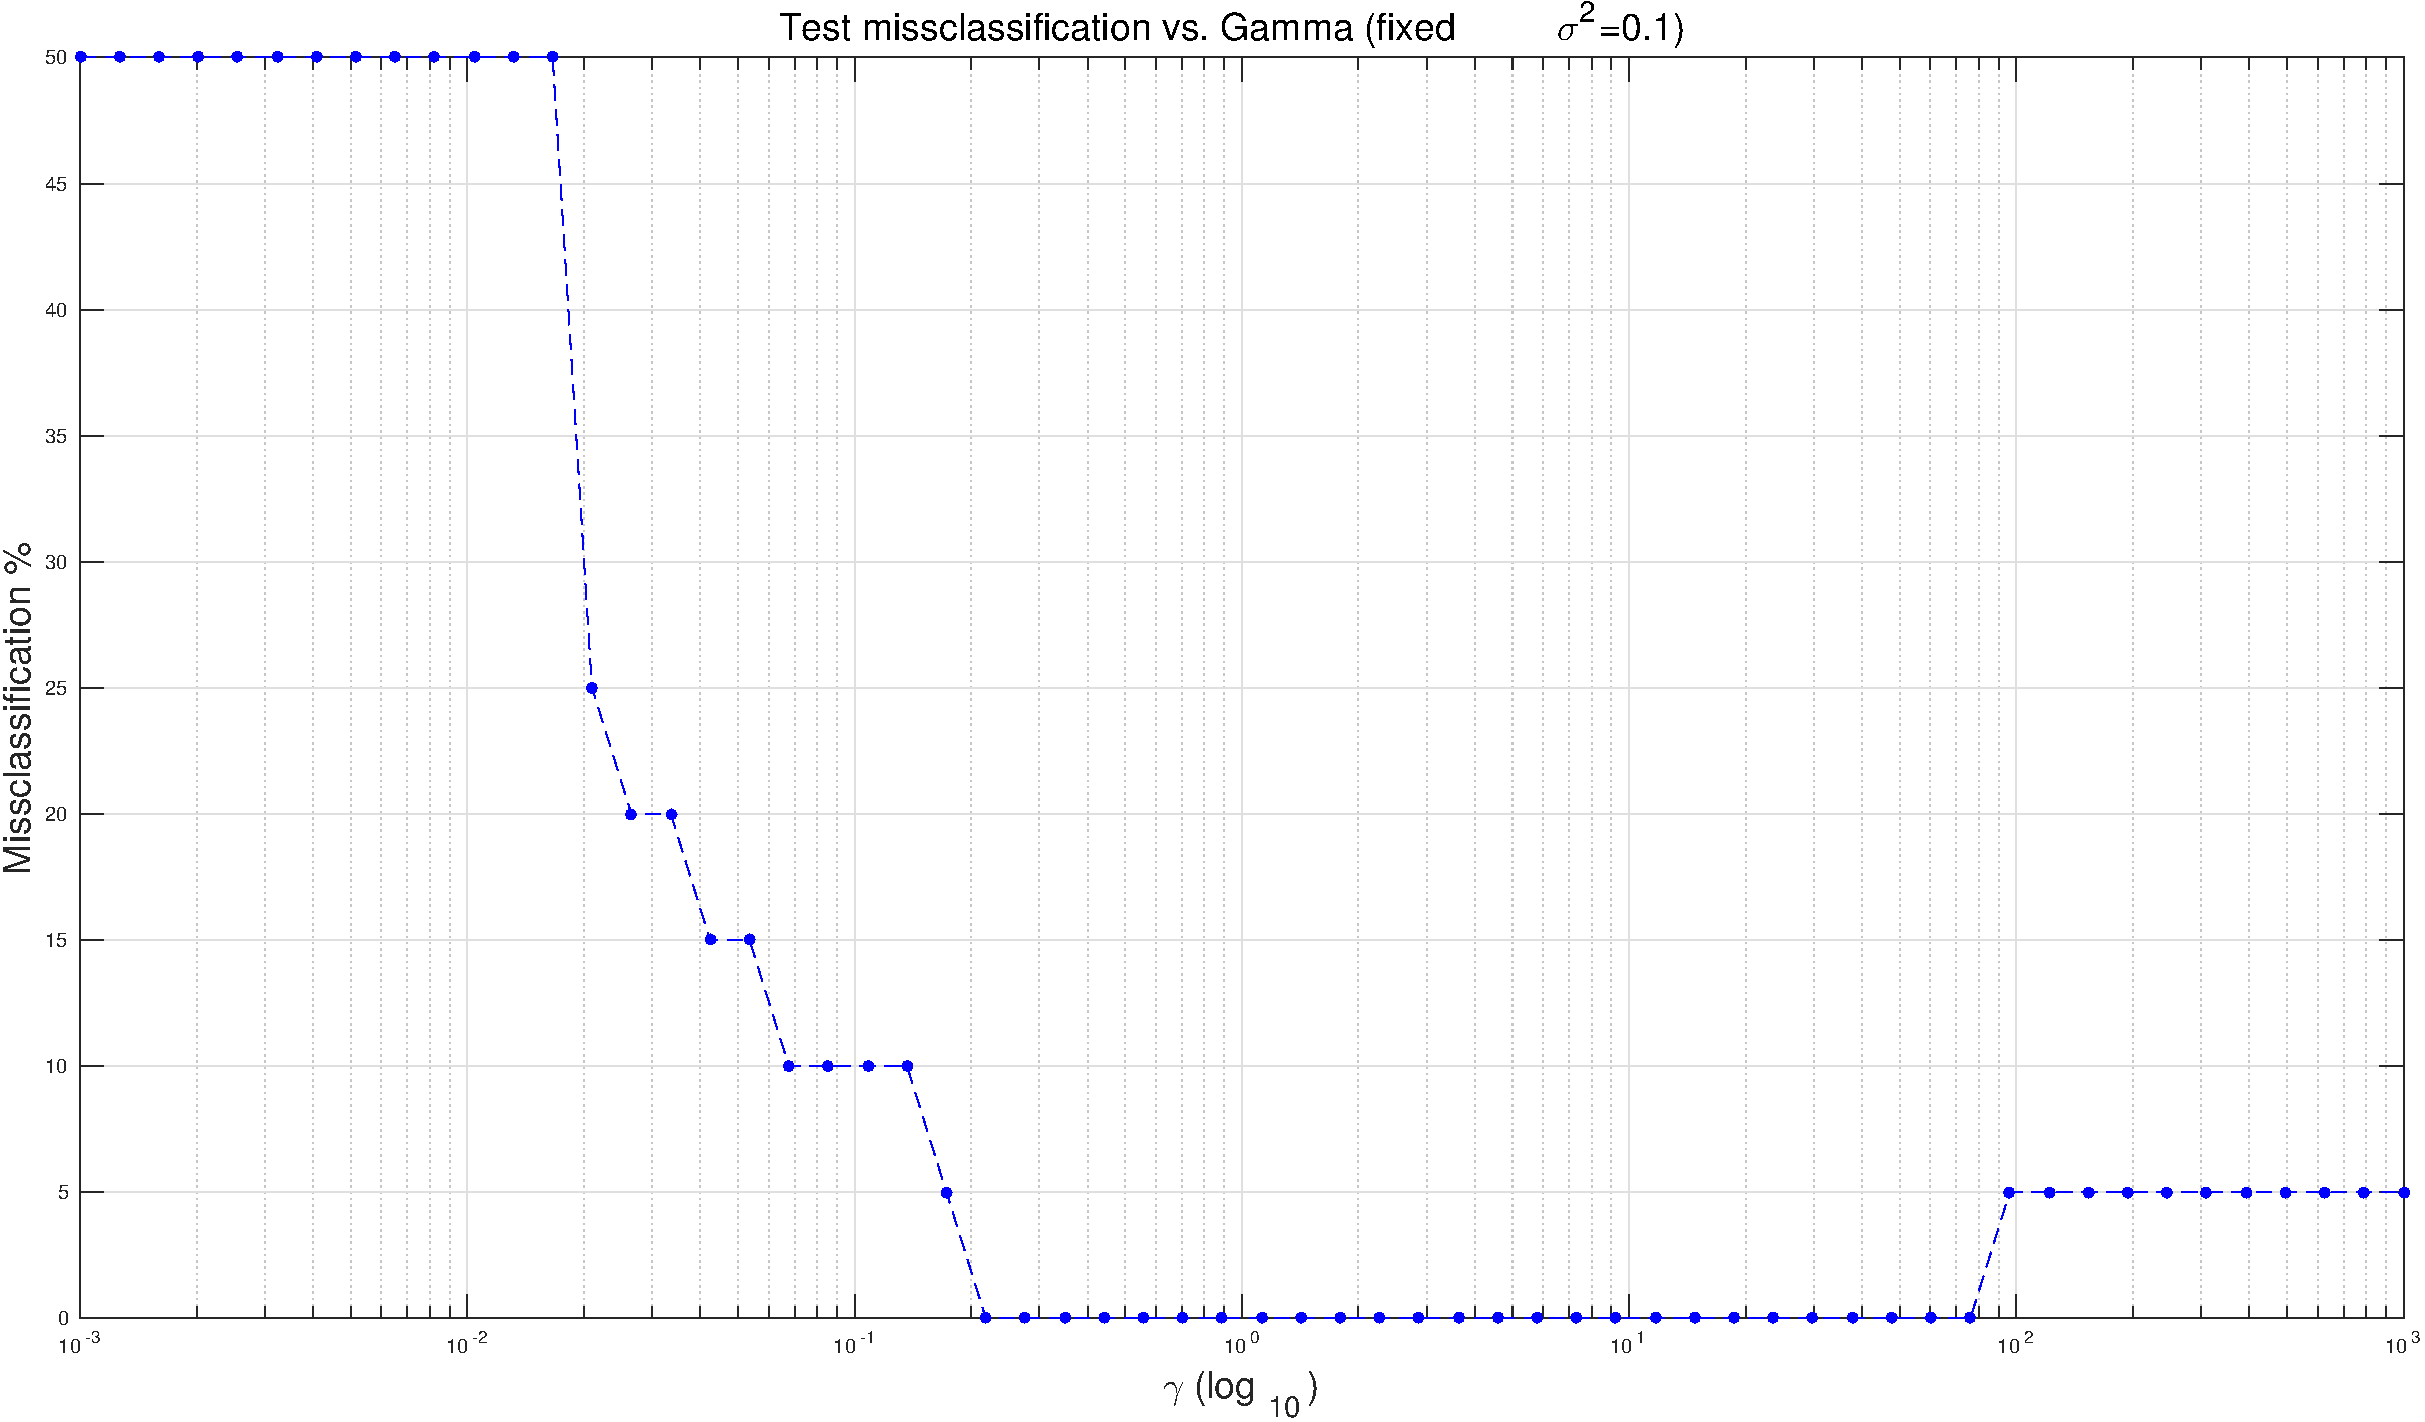
\includegraphics[scale=.40]{rbf_gamma.pdf}
    \caption{Tuning of parameter $\gamma$ for fixed $\sigma^2=0.1$}
    \label{fig:rbf_gamma}
\end{figure}

\subsection{Choice of hyper-parameters}
\subsubsection{Validation set}

For this section, I created a validation set for the Iris dataset
consisting of a fifth of the total number of observations used in the
previous section to train the classifier. Here is the code for that
purpose:

\begin{lstlisting}
idx = randperm(size(X,1));
Xtrain = X(idx(1:80),:);
Ytrain = Y(idx(1:80),:);
Xval = X(idx(81:100),:);
Yval = Y(idx(81:100),:);
\end{lstlisting}

In order to choose appropriate values for the hyper parameters, I
trained classifiers using a log grid of $\sigma^2$ and $\gamma$, and
computed the test error on the validation set as follow:

\begin{lstlisting}
% Searching sigma space for a good value (good generalization on test set)
sig2list=logspace(-3,3,60); errsiglist=[]; gam = 1;
for sig2=sig2list,
    [alpha,b] = trainlssvm({Xtrain,Ytrain,'c',gam,sig2,'RBF_kernel'});
    % Obtain classification of test set using trained classifier
    estYval = simlssvm({Xtrain,Ytrain,'c',gam,sig2,'RBF_kernel'}, {alpha,b}, Xval);
    err = sum(estYval~=Yval); errsiglist = [errsiglist; err]; 
end

% Searching sigma space for a good value (good generalization on test set)
sig2 = 0.1; gamlist=logspace(-3,3,60); type='c'; errgamlist=[];
for gam=gamlist,
    [alpha,b] = trainlssvm({Xtrain,Ytrain,'c',gam,sig2,'RBF_kernel'});
    % Obtain classification of test set using trained classifier
    estYval = simlssvm({Xtrain,Ytrain,'c',gam,sig2,'RBF_kernel'}, {alpha,b}, Xval);
    err = sum(estYval~=Yval); errgamlist = [errgamlist; err];
end
\end{lstlisting}

The figure \ref{fig:hyperparams_choice1} gives an overview of the
misclassification rate for different values of the
hyperparameters. One can observe that the ``optimal'' range in which
to select the parameters if slightly different than that of the
previous section. Since we have defined a different set to test the
performance and given that we have few observations (\textless 100),
we can expect variance in the evaluation of test error. The specific
values obtained being contingent upon the random split of the dataset
between training and validation.

Importantly, one should not re-use the validation set to estimate the
generalization of the model but rather should set aside a test set
(untouched during the whole training). Indeed using the same
validation set would likely induce an optimisticly biased
generalization estimation (memorization of the dataset).

\begin{figure}[H]
    \centering
    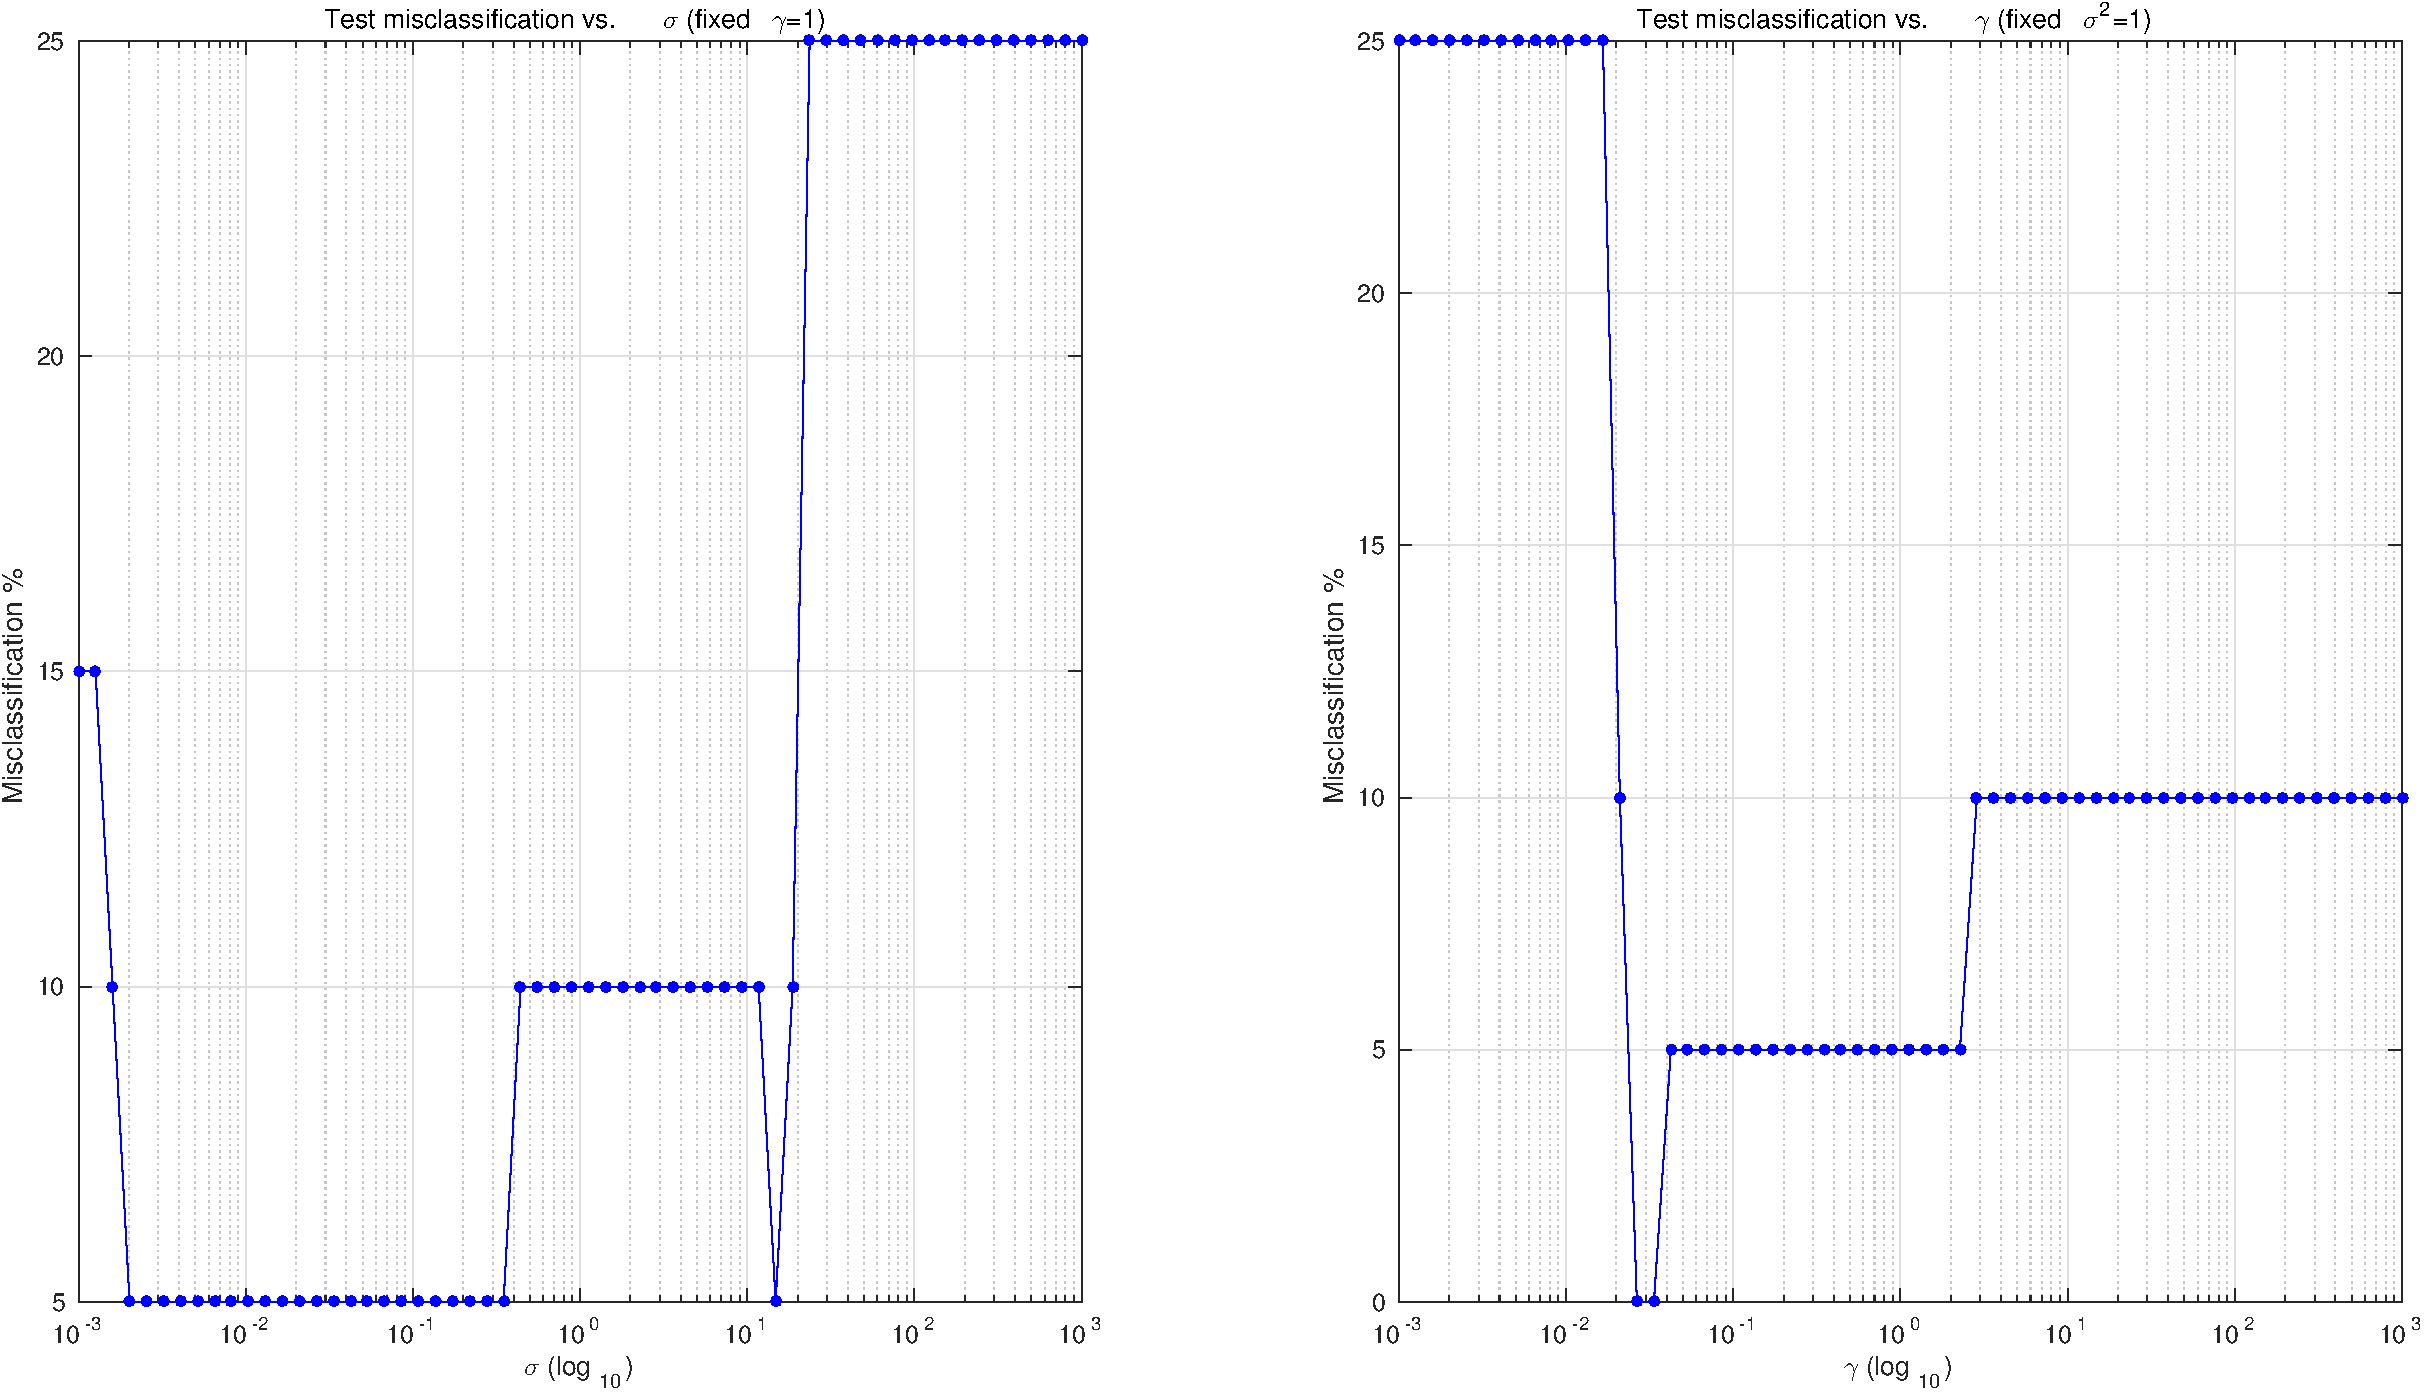
\includegraphics[scale=.40]{hyperparams_choice1.pdf}
    \caption{Tuning of parameter $\gamma$ and $\sigma^2$ based on the
      validation set}
    \label{fig:hyperparams_choice1}
\end{figure}

\subsubsection{Cross validation}

Cross validation is a common technique in statistics to help remove
the variance in the parameters estimation due to the random split of
the dataset between training set and validation set. In smaller
datasets, high variance can ensue from validating a model given one
split, or another split. By systematically building multiple splits,
training and validating the models, one can obtain a more averaged test
error.

In this section, we used 10 fold cross validation, which consists in
creating 10 different splits of the original dataset. For each split,
90 percent of the data is used to train a model, and 10 percent is
used for validation. At each new split, there is no overlap of the
validation cases with previous validation cases, so the whole training
dataset is surveyed. The validation errors are averaged accross the 10
splits to obtain the average validation error on the whole training
dataset.

For the LOOCV, the procedure is the same, but only a single datapoint
is kept at each split to validate the model. The procedure is thus
repeated n times (n being the number of observations).

These are the results for the Iris dataset:
\begin{verbatim}
>> crossvalidate({X, Y, 'c', gam, sig2, 'RBF_kernel'}, 10, 'misclass');
    0.0600

>> leaveoneout({X, Y, 'c', gam, sig2, 'RBF_kernel'}, 'misclass');
    0.0500
\end{verbatim}

The LOOCV can be computationally expensive on large datasets, though
there exists exceptions to that (eg, in the case of linear regression,
it is possible to compute the LOOCV using a simple analytical
formula). The LOOCV is also known to have more bias since it uses
systematically ``almost'' the whole dataset. It can however be useful
on datasets containing very few observations.

\subsubsection{Optimization techniques}

In this section, we try to optimize the hyperparameters using global
optimization techniques. The results are reported in
\ref{table:hyperparamstuning}. One thing to note is the stochasticity
of the search process. Accross multiple runs (3 illustrated in the
table), the results are widely variable in terms of the selected
hyperparameters. The hyperparameter $\sigma^2$ however falls into the
range previously established. $\gamma$ is a bit higher in magnitude
than expected using the previous approach.

Another important distinction to make here, is that although the
formulation of the SVM problem is indeed convex, we now are faced with
a problem of hyperparameter selection, which is non-convex, and many
local minima are now possible. Hence the technique \emph{csa} and
\emph{ds} are global optimization techniques that can help with the
search (though without garantees of locating a global minimum). In a
first step, those techniques will act to select in the landscape a
place to start the search, which is then finalized using a
\emph{simplex} approach, or a pre-defined \emph{searchgrid}. This
explains the variability in the returned \emph{optimized} parameters.

\begin{lstlisting}
% coupled simulated annealing
model_csa = {X, Y, 'c', [], [], 'RBF_kernel', 'csa'};
[gam1, sig21, cost1] = tunelssvm(model_csa, 'simplex', 'crossvalidatelssvm', {10, 'misclass'});
[gam2, sig22, cost2] = tunelssvm(model_csa, 'gridsearch', 'crossvalidatelssvm', {10, 'misclass'});
% randomized directional search
model_ds = {X, Y, 'c', [], [], 'RBF_kernel', 'ds'};
[gam3, sig23, cost3] = tunelssvm(model_ds, 'simplex', 'crossvalidatelssvm', {10, 'misclass'});
[gam4, sig24, cost4] = tunelssvm(model_ds, 'gridsearch', 'crossvalidatelssvm', {10, 'misclass'});
\end{lstlisting}

\begin{table}[H]
  \centering
  \begin{tabular}{cl|l|l|l|l|l|l|l|l|l|}
    \cline{3-11}
    \multicolumn{1}{l}{}                       &            & \multicolumn{3}{c|}{Run 1}   & \multicolumn{3}{c|}{Run 2}   & \multicolumn{3}{c|}{Run 3}   \\ \cline{3-11} 
    \multicolumn{1}{l}{}                       &            & $\gamma$ & $\sigma^2$ & Cost & $\gamma$ & $\sigma^2$ & Cost & $\gamma$ & $\sigma^2$ & Cost \\ \hline
    \multicolumn{1}{|c|}{\multirow{2}{*}{CSA}} & simplex    & 2.14     & 1.32       & 0.04 & 3670     & 0.06       & 0.03 & 123.84   & 0.03       & 0.03 \\ \cline{2-11} 
    \multicolumn{1}{|c|}{}                     & gridsearch & 176.24   & 0.02       & 0.03 & 0.65     & 0.09       & 0.04 & 0.11     & 0.73       & 0.04 \\ \hline
    \multicolumn{1}{|c|}{\multirow{2}{*}{DS}}  & simplex    & 0.93     & 6.66       & 0.04 & 7.60     & 2.37       & 0.05 & 4.54     & 1.27       & 0.05 \\ \cline{2-11} 
    \multicolumn{1}{|c|}{}                     & gridsearch & 0.05     & 0.93       & 0.03 & 41.96    & 0.21       & 0.03 & 0.05     & 0.21       & 0.03 \\ \hline
  \end{tabular}
  \caption{Hyperparameters tuning}
  \label{table:hyperparamstuning}
\end{table}

\subsubsection{ROC}

Receiver Operating Characteristics are a very popular tool to assess
the quality of a classifier in terms of predictive power. They can be
thought of as continuously evaluated (by changing the decision
treshold) contingency tables. 

One should not build ROC using the training dataset for the same
reason that you don't assess the quality of a model based on the
training dataset. Many techniques systematically minimize the error
between the model and the training observations (eg, least mean
squares). Thus the ROC curve can be made really good by just
``memorizing'' the dataset, without any regard for good
generalization.

\section{Applications} 

\subsection{Ripley dataset}
\subsubsection{Data visualization}

A scatterplot of the training dataset is shown on figure
\ref{fig:ripley_scatter}. The 2 categories seem to be overlapping
quite a bit, and are separated (though not clearly) on the vertical
axis, with the upper part of the scatterplot consisting mostly of one
category (here ``1''), and the bottom part of the scatterplot, with
the other category (here ``-1''). Further, it would seem that the
``-1'' category has 2 centroid, one around X=-0.75, and the other
around X=0.4. The same observation can be made for the category ``1'',
though the separation between the 2 centroids is less pronouced. 

Intuitively, it would seem that a linear classifier may do a good job
at classifying observations that are further appart to the Y=0.5 axis,
but will perform poorly close to that region due to considerable
overlap.

\begin{figure}[H]
    \centering
    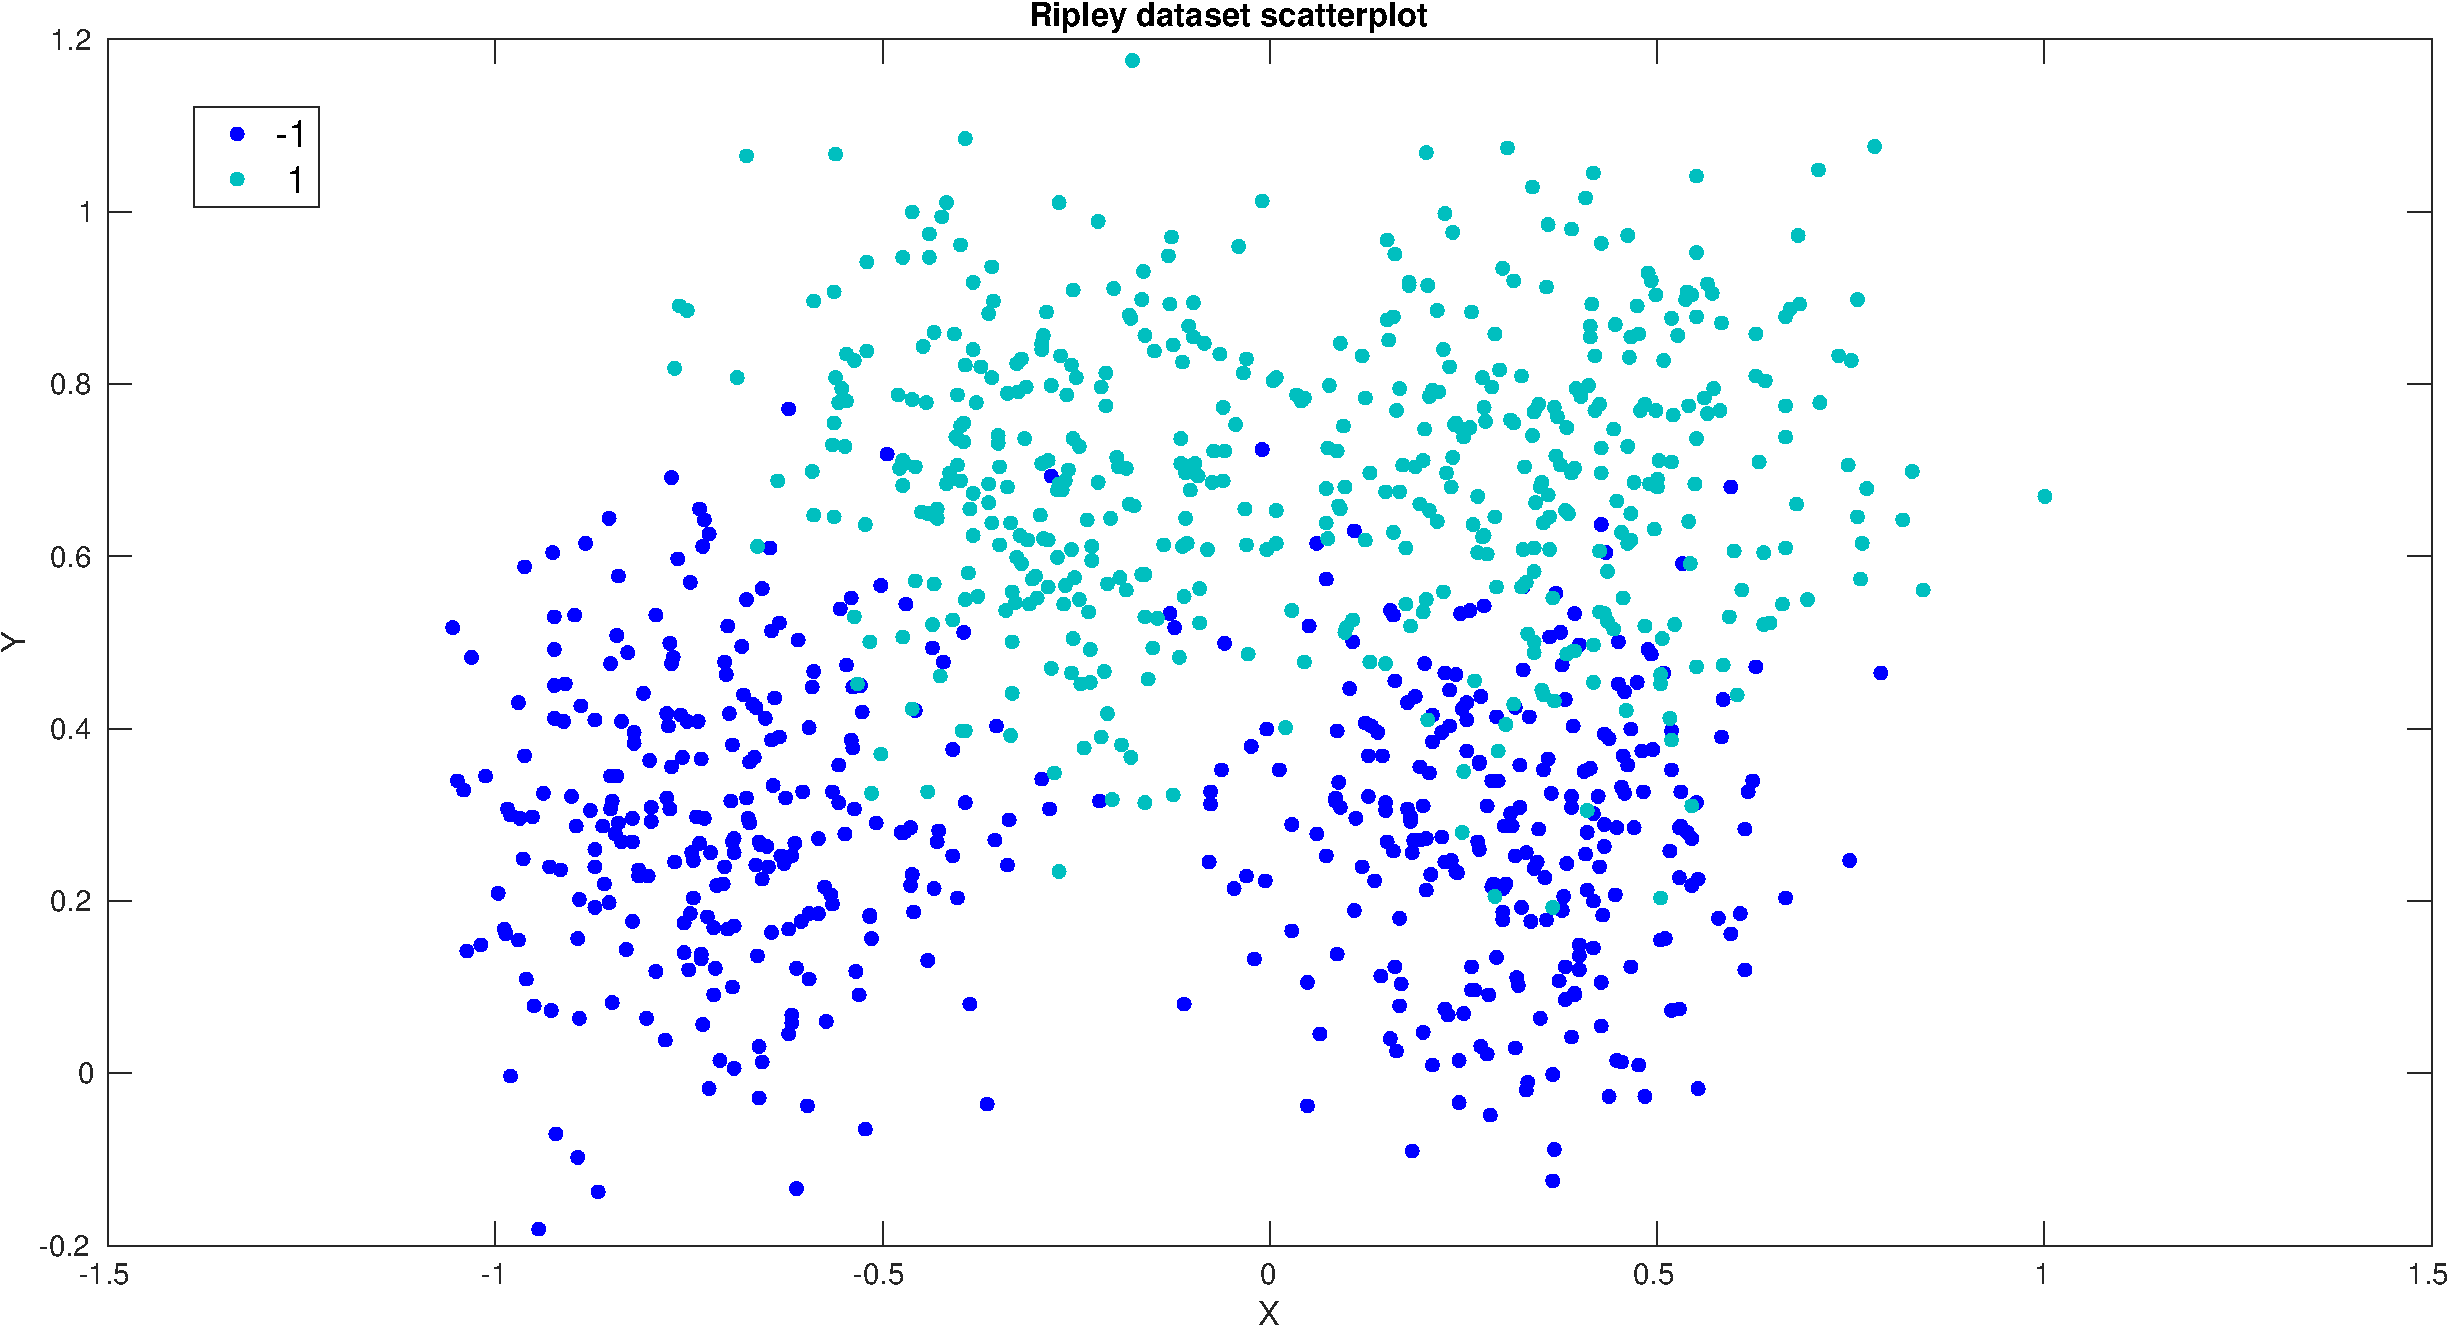
\includegraphics[scale=.40]{ripley_scatter.pdf}
    \caption{Ripley dataset scatterplot by group}
    \label{fig:ripley_scatter}
\end{figure}

\subsubsection{Linear model}

In order to test the intuition about the linear separability, I built
a LS-SVM model that has a polynomial kernel of degree 1. The resulting
classifier can be seen on the left-hand side of figure
\ref{fig:ripley_lin_rbf}

\begin{lstlisting}
gamlist=logspace(-4,3); type='c'; errlist=[];

for gam=gamlist,
    [alpha,b] = trainlssvm({Xt,Yt,type,gam,[],'lin_kernel'});
    [Yht, Zt] = simlssvm({Xt,Yt,type,gam,[],'lin_kernel'}, {alpha,b}, X);
    err = sum(Yht~=Y); errlist = [errlist; err];
end
[min, index] = min(errlist);
plotlssvm({Xt,Yt,type,gamlist(index),[],'lin_kernel','preprocess'},{alpha,b});
\end{lstlisting}

\subsubsection{RBF model}

The resulting classifier can be seen on the right-hand side of figure
\ref{fig:ripley_lin_rbf}

\begin{lstlisting}
model_csa = {Xt, Yt, 'c', [], [], 'RBF_kernel', 'csa'};
[gam, sig2, cost] = tunelssvm(model_csa, 'simplex', 'crossvalidatelssvm', {10, 'misclass'});

[alpha,b] = trainlssvm({Xt,Yt,'c',gam,sig2,'RBF_kernel'});
estYval = simlssvm({Xt,Yt,'c',gam,sig2,'RBF_kernel'}, {alpha,b}, X);
err = sum(estYval~=Y);
plotlssvm({Xt,Yt,type,gam,sig2,'RBF_kernel','preprocess'},{alpha,b});
\end{lstlisting}

\begin{figure}[H]
    \centering
    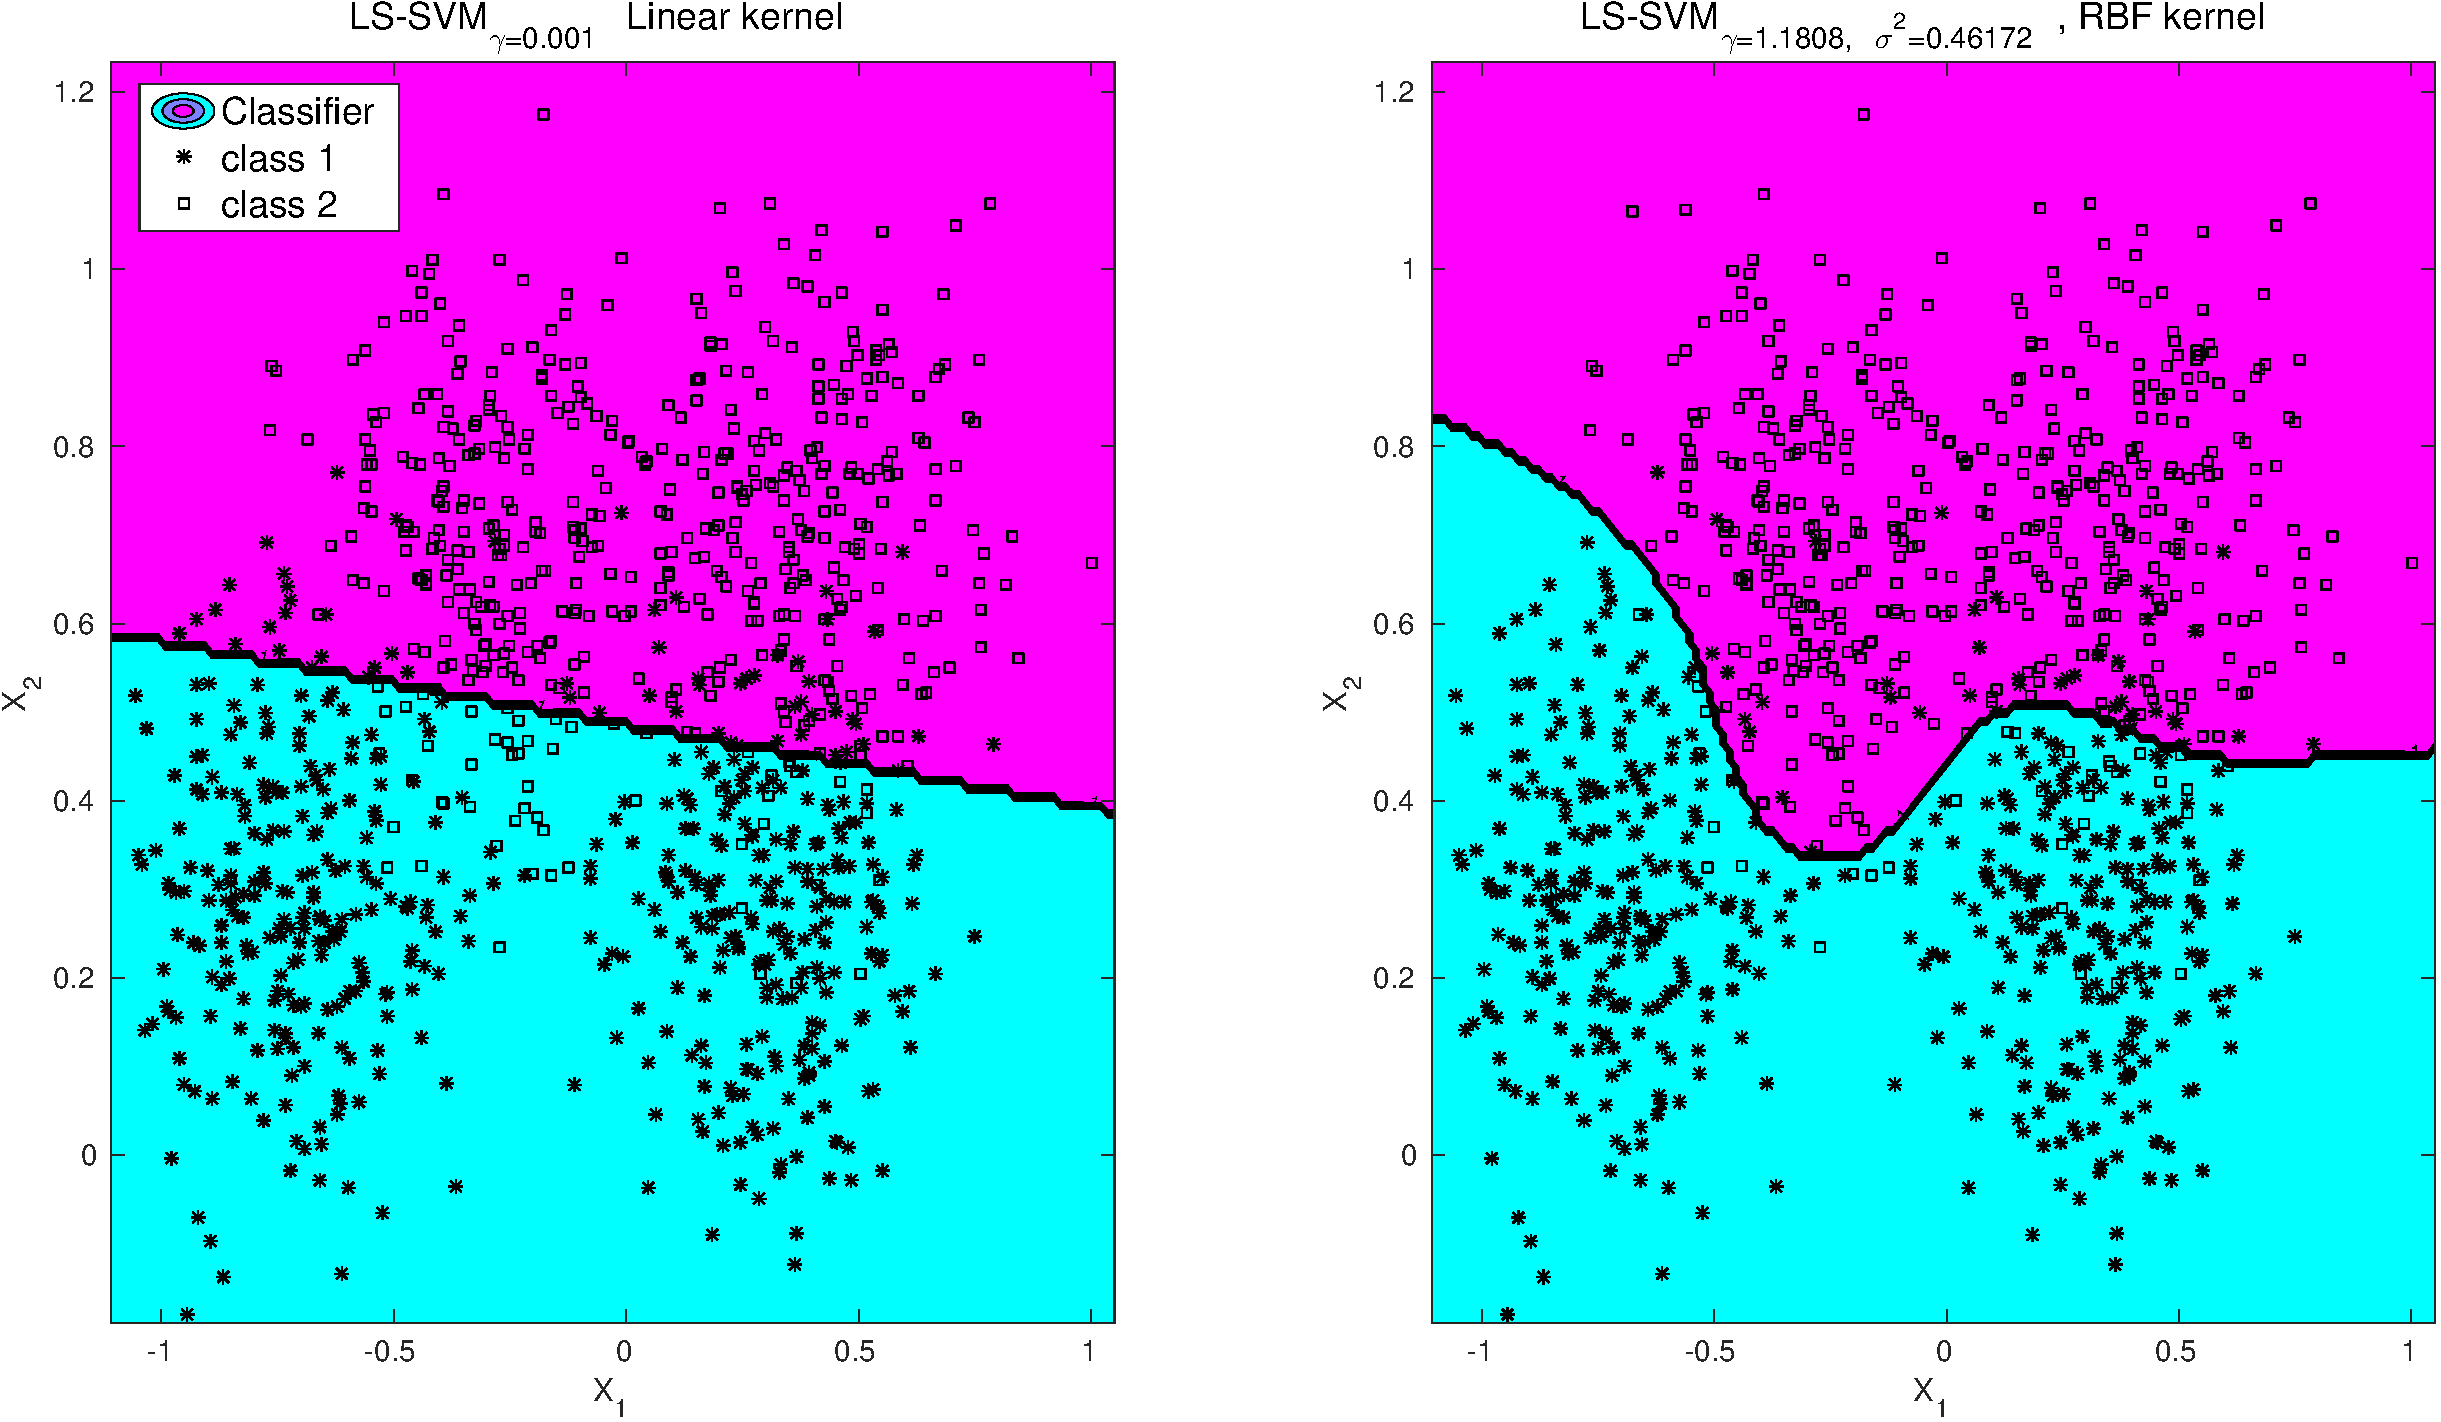
\includegraphics[scale=.40]{ripley_lin_RBF.pdf}
    \caption{Ripley dataset, left linear kernel, right RBF kernel}
    \label{fig:ripley_lin_rbf}
\end{figure}

\subsubsection{ROC curves}

\begin{figure}[H]
    \centering
    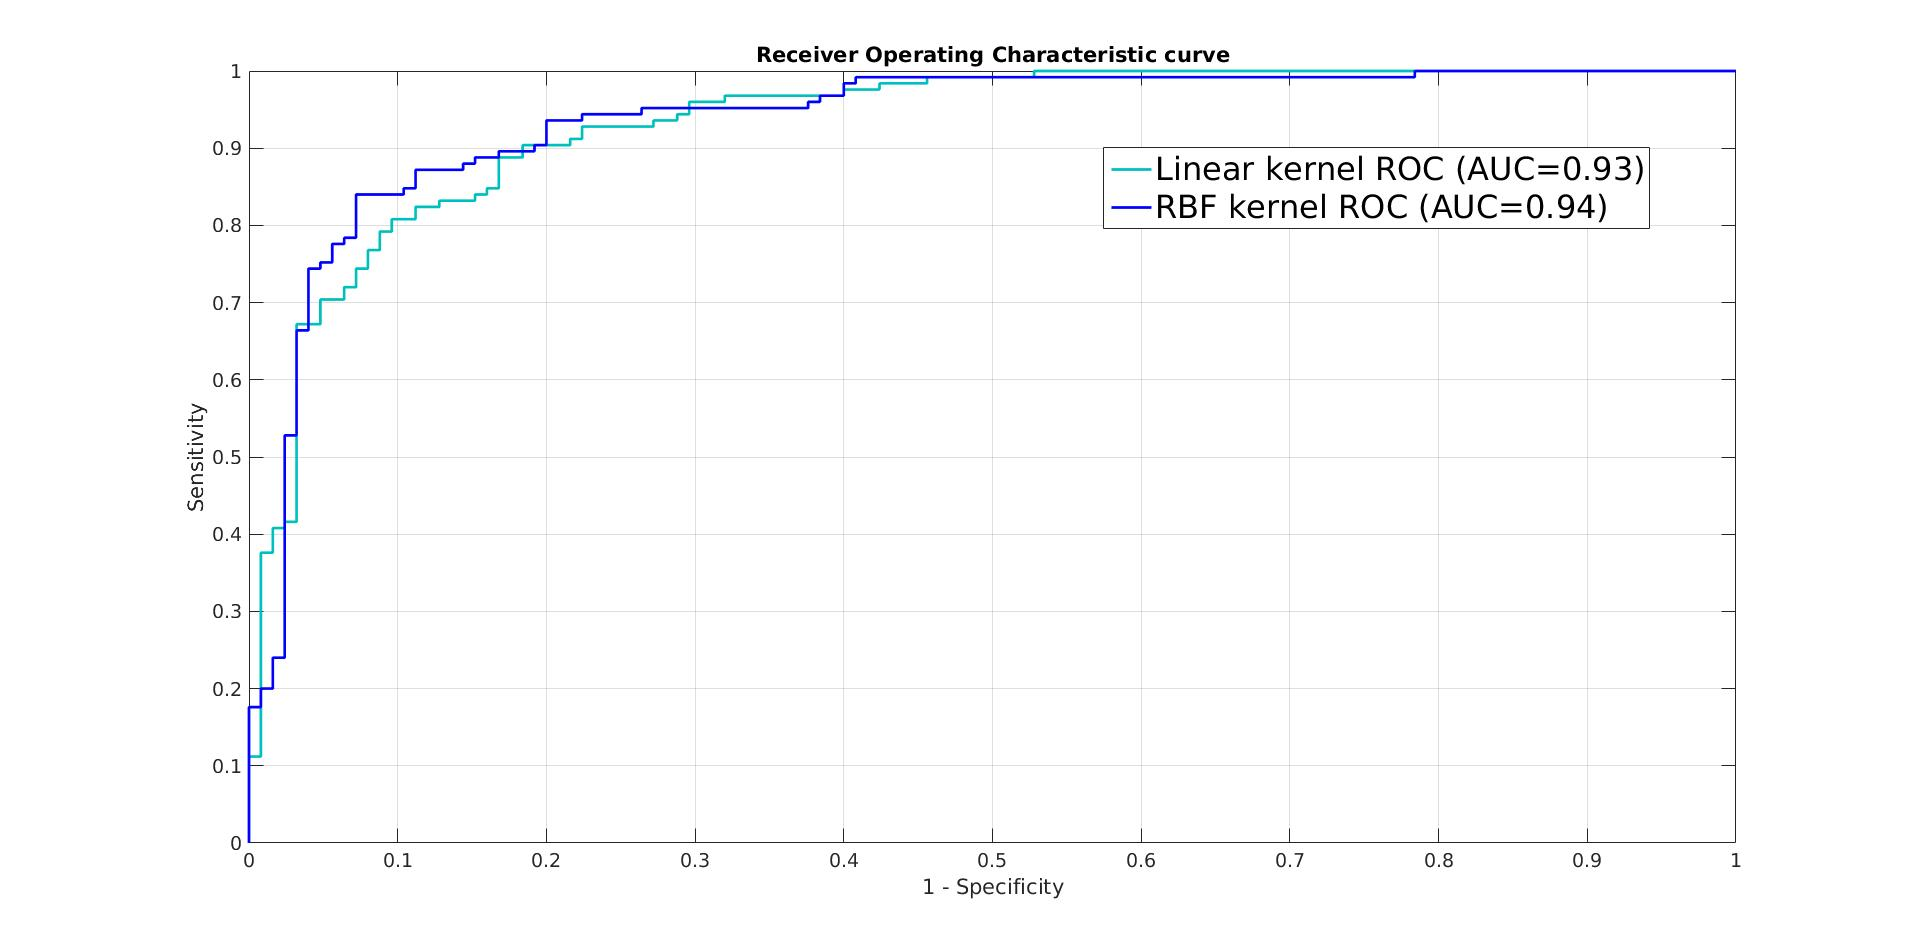
\includegraphics[scale=.20]{ripley_roc.jpg}
    \caption{ROC of both classifiers}
    \label{fig:ripley_rbf}
\end{figure}

\subsubsection{Final model selection}
As illustrated by the ROC curves, the performance on the test set of
the RBF classifier is only marginally superior. The Ripley dataset
consists of overlapping gaussian distributions, so using a simpler
model that incorporates a linear classifier could make sense here, but
I would still favor the RBF kernel model given the knowledge of the
dataset's structure.

\subsection{Breast cancer dataset}

\subsubsection{Data visualization}

This dataset contains significantly more variables than the previous
one and cannot be easily plotted for interpretation. A quick boxplot
of the 30 variables reveals a lot of variance in the scale, so I
performed dimensionality reduction using Principal component analysis
with scaling using variance. The results are shown on figure
\ref{fig:breast_pcaviz}. From the importance of principal component
plot, one can see that the first 3 PC explain a large amount of the
variability in the data. Linear separability seems to appear when
plotting the data using 3PC and 2PC. 

\begin{figure}[H]
    \centering
    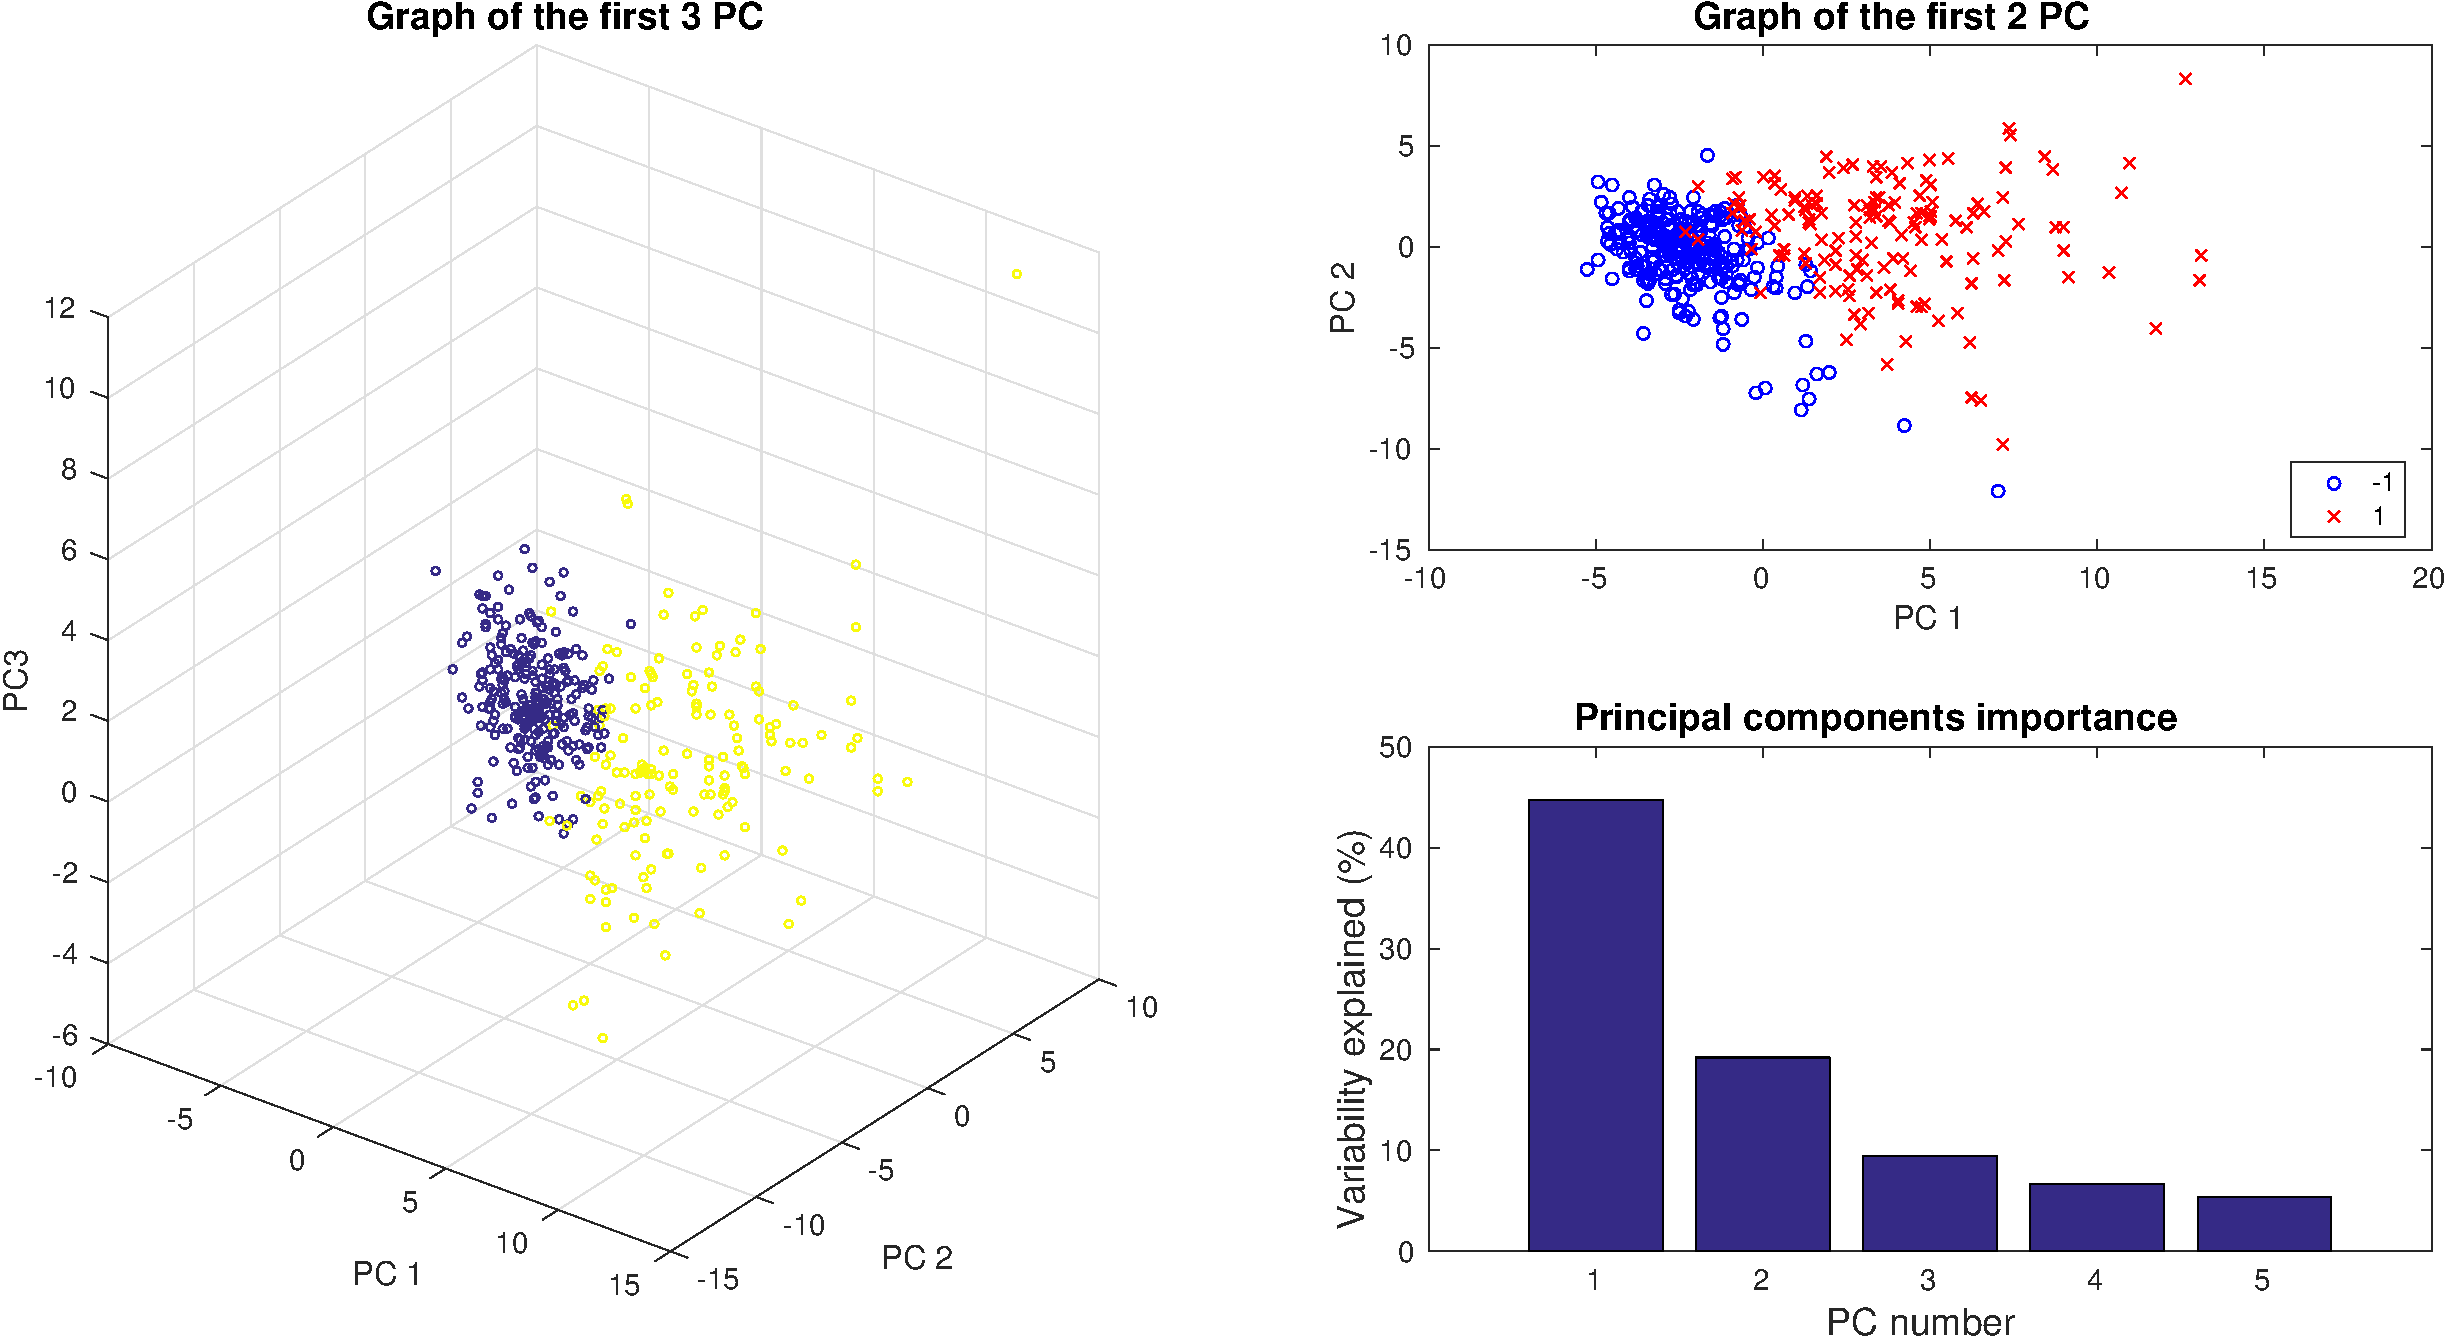
\includegraphics[scale=.40]{breast_pcaviz.pdf}
    \caption{Principal components analysis and visualization}
    \label{fig:breast_pcaviz}
\end{figure}

\subsubsection{Linear model}

The reported performance of the classification for the test set is: 96.4\%

\begin{lstlisting}
gamlist=logspace(-3,3); type='c'; errlist=[];

for gam=gamlist,
    [alpha,b] = trainlssvm({trainset,labels_train,type,gam,[],'lin_kernel'});
    [Yht, Ylin] = simlssvm({trainset,labels_train,type,gam,[],'lin_kernel'}, {alpha,b}, testset);
    err = sum(Yht~=labels_test); errlist = [errlist; err];
end
[min, index] = min(errlist);
[Yht, Ylin] = simlssvm({trainset,labels_train,type,gamlist(index),[],'lin_kernel'}, {alpha,b}, testset);
perf_lin = (1-errlist(index)/numel(labels_test))*100;
\end{lstlisting}

\subsubsection{RBF model}

The reported performance of the classification for the test set is: 97.6\%

\begin{lstlisting}
model_csa = {trainset, labels_train, 'c', [], [], 'RBF_kernel', 'csa'};
[gam, sig2, cost] = tunelssvm(model_csa, 'simplex', 'crossvalidatelssvm', {10, 'misclass'});

[alpha,b] = trainlssvm({trainset,labels_train,'c',gam,sig2,'RBF_kernel'});
[estYval, YRBF] = simlssvm({trainset,labels_train,'c',gam,sig2,'RBF_kernel'}, {alpha,b}, testset);
err = sum(estYval~=labels_test); perf_rbf = (1-err/numel(labels_test))*100;
\end{lstlisting}

\subsubsection{ROC curves}

\begin{figure}[H]
    \centering
    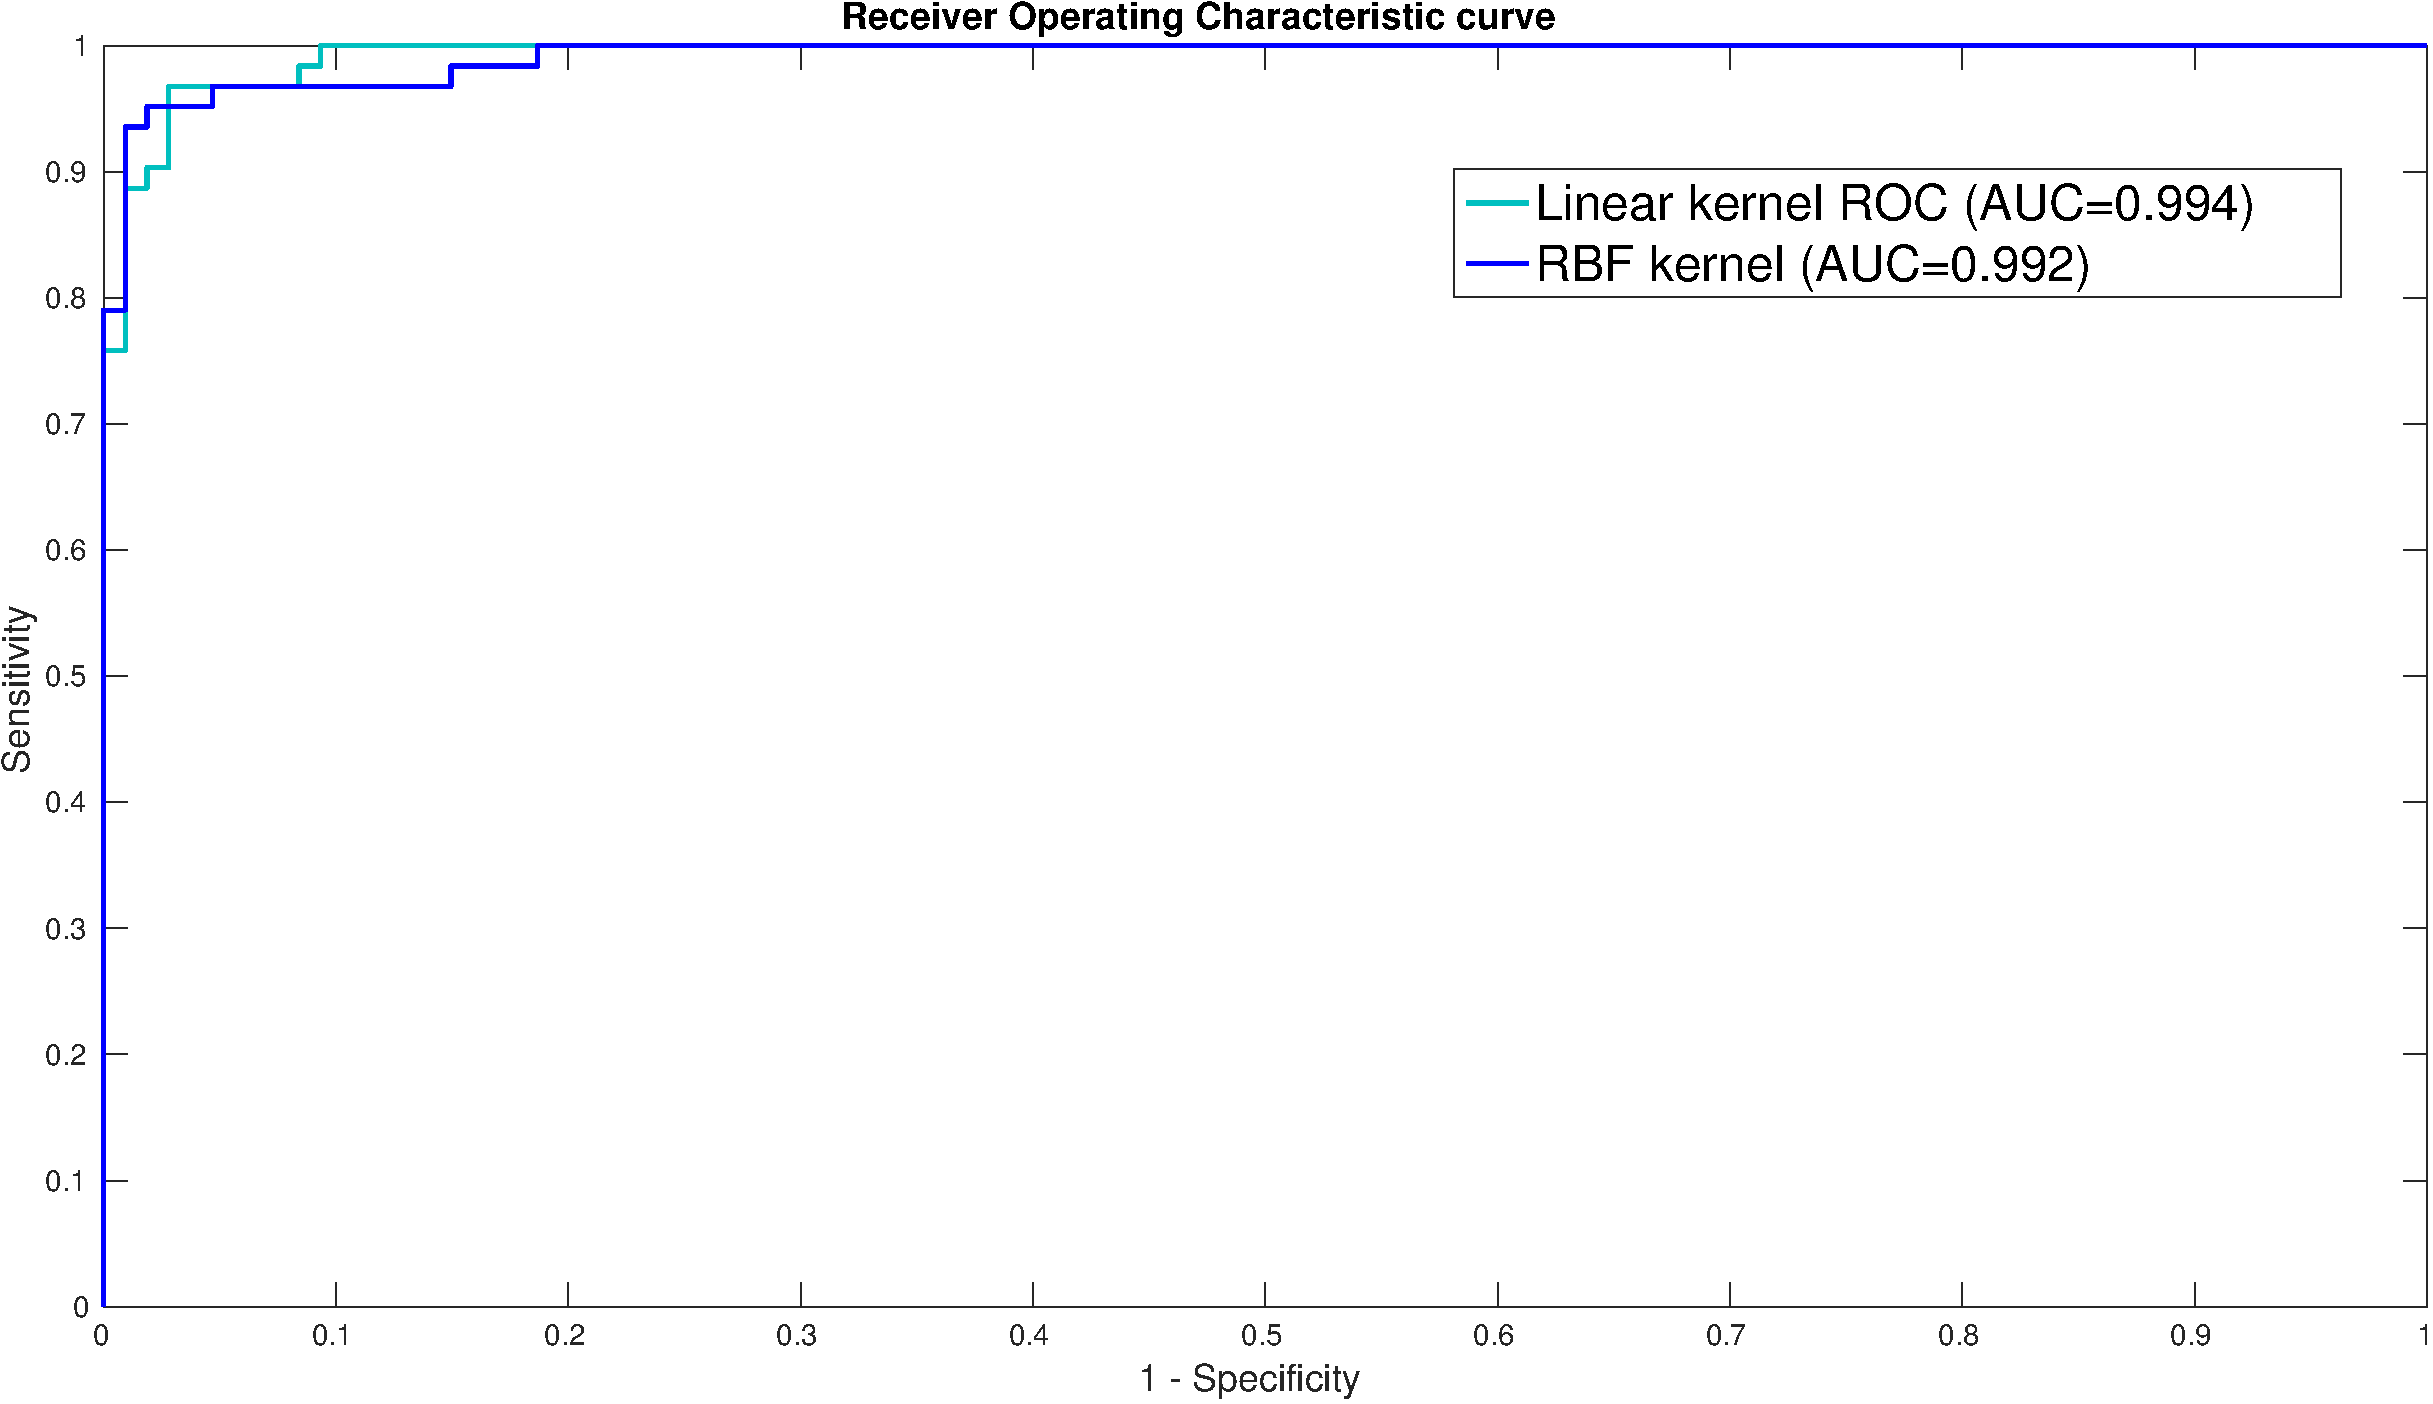
\includegraphics[scale=.40]{breast_ROC.pdf}
    \caption{ROC of both classifiers}
    \label{fig:breast_ROC}
\end{figure}

\subsubsection{Final model selection}

Similarly to section 4.1.5, we see that there isn't much support for
and RBF kernel based modelling for this dataset. As illustrated by the
ROC curves, the performance on the validation set of the RBF
classifier is only marginally superior. This analysis is comforted by
the fact that visually we can see a linear separability in the
principal components plot.

\subsection{Diabetes database}

\subsubsection{Data visualization}

Using the same approach as in the previous section for the
visualization with a PC decomposition, we cannot see a clear linear
separability between the datapoints (see figure
\ref{fig:diabetes_pcaviz}). 

\begin{figure}[H]
    \centering
    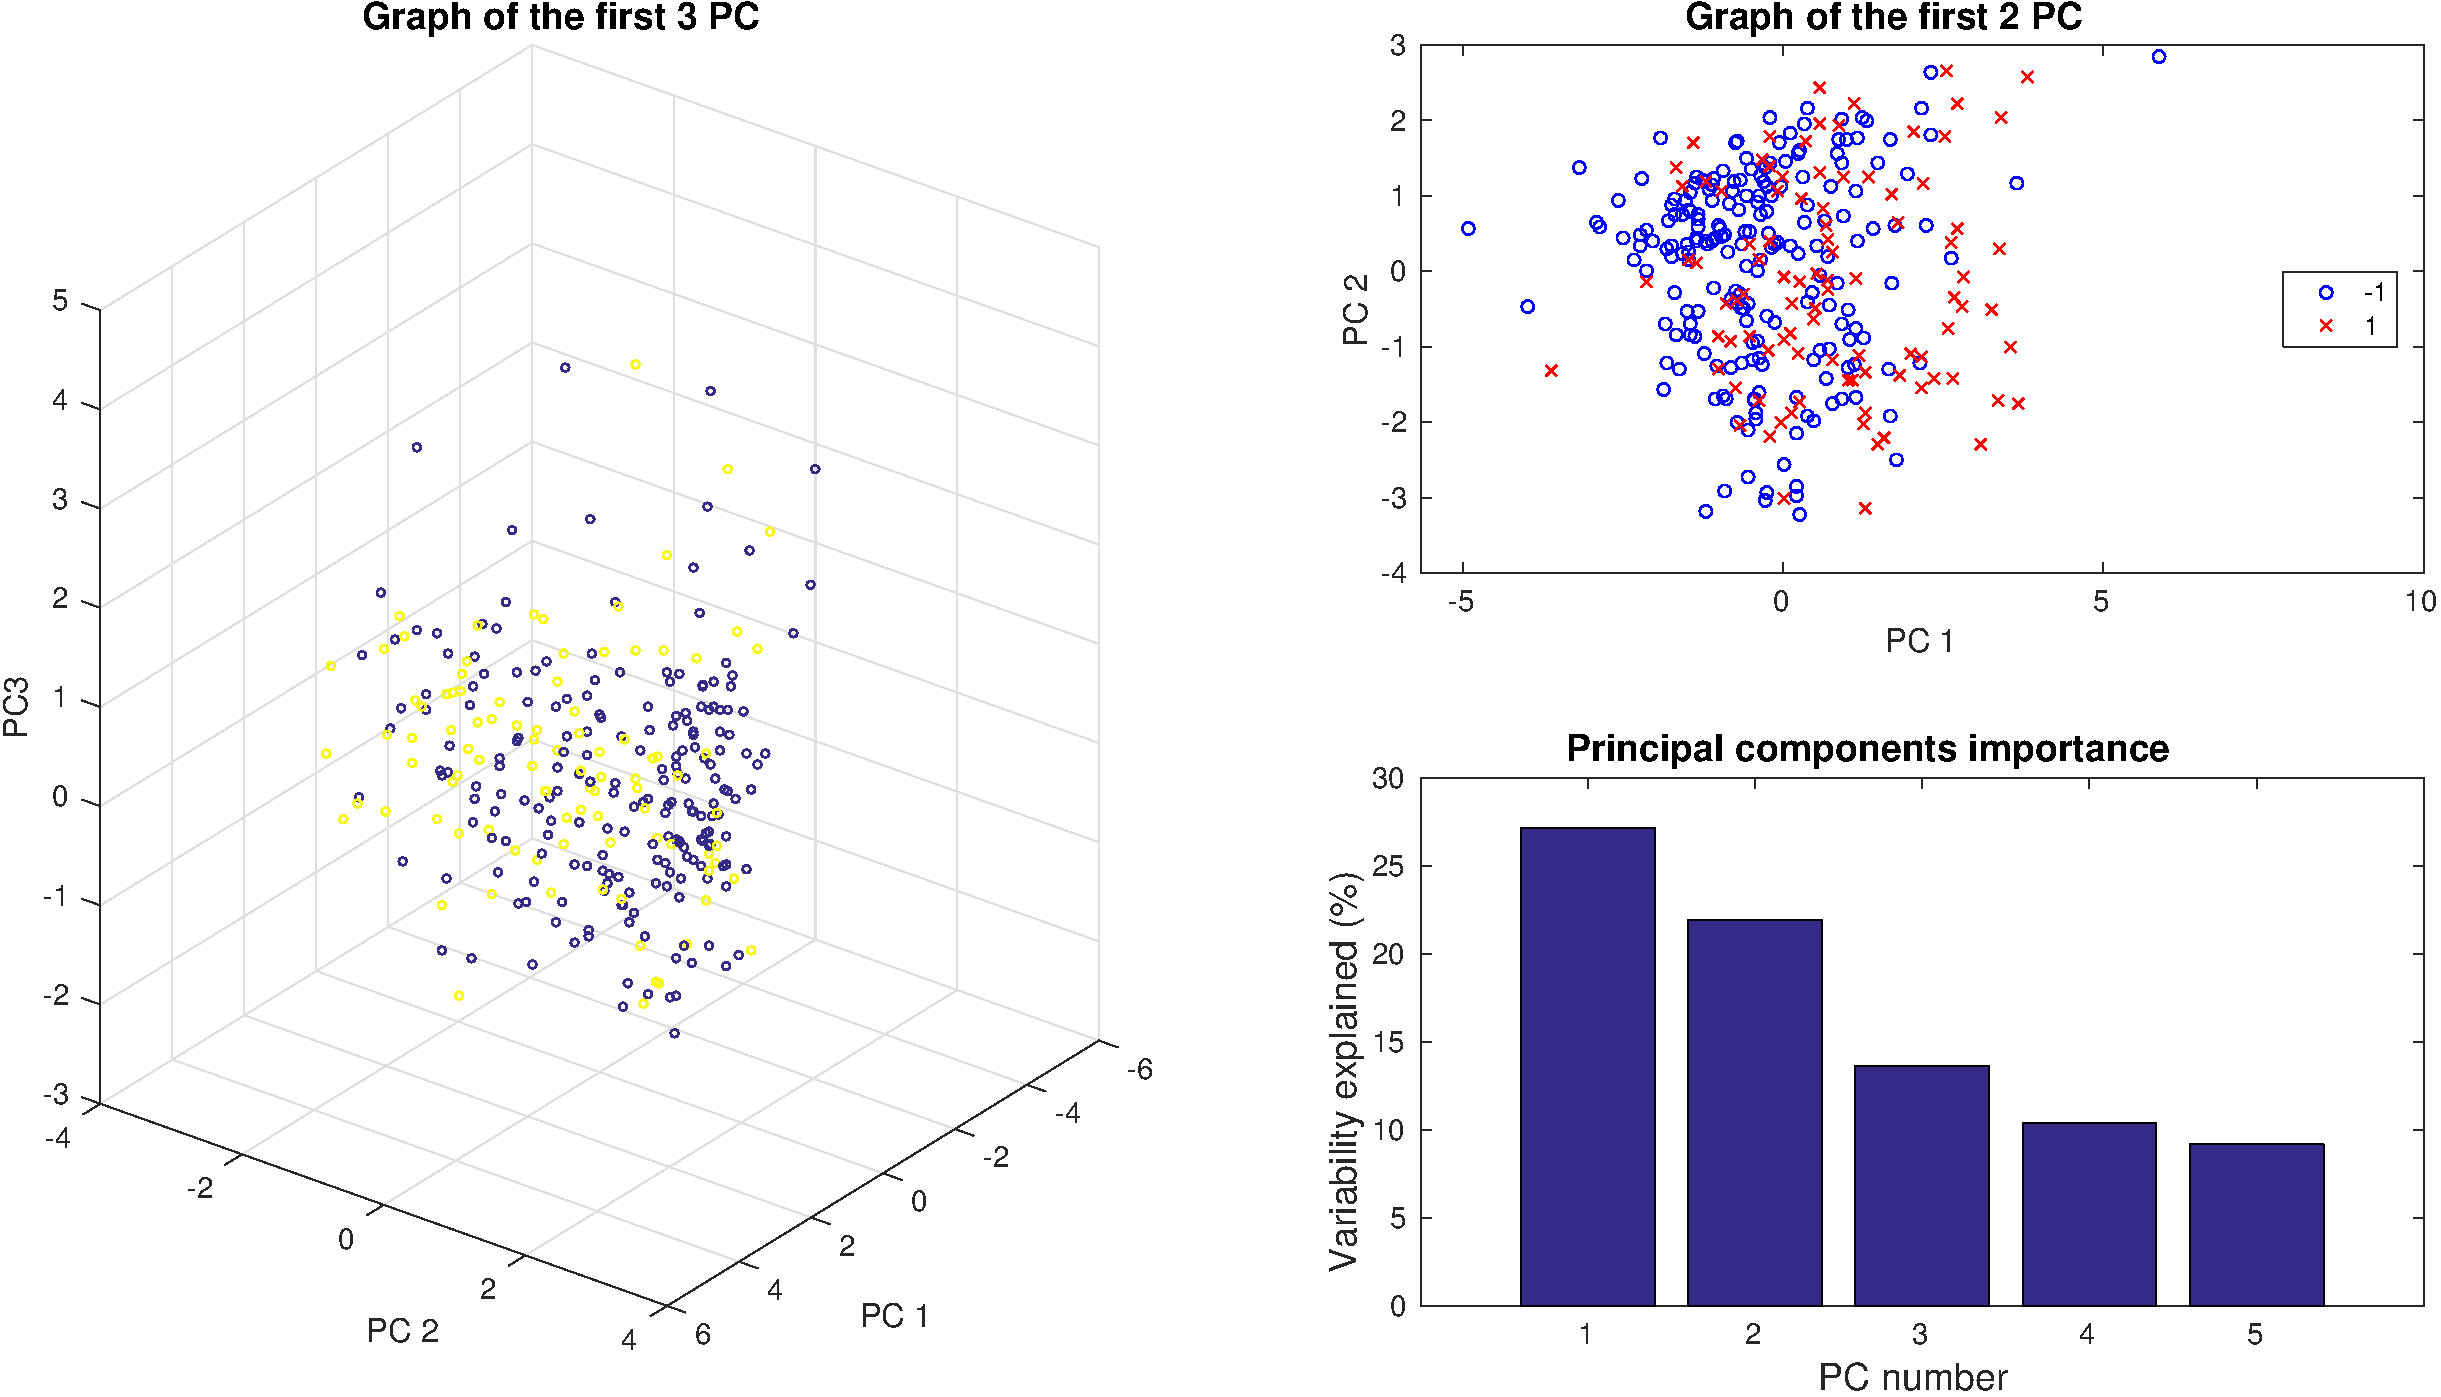
\includegraphics[scale=.40]{diabetes_pcaviz.pdf}
    \caption{Principal components visualization}
    \label{fig:diabetes_pcaviz}
\end{figure}

\subsubsection{Linear model}

The reported performance of the classification for the test set is: 79.8\%

\begin{lstlisting}
gamlist=logspace(-3,3); type='c'; errlist=[];

for gam=gamlist,
    [alpha,b] = trainlssvm({trainset,labels_train,type,gam,[],'lin_kernel'});
    [Yht, Ylin] = simlssvm({trainset,labels_train,type,gam,[],'lin_kernel'}, {alpha,b}, testset);
    err = sum(Yht~=labels_test); errlist = [errlist; err];
end
[min, index] = min(errlist);
[Yht, Ylin] = simlssvm({trainset,labels_train,type,gamlist(index),[],'lin_kernel'}, {alpha,b}, testset);
perf_lin = (1-errlist(index)/numel(labels_test))*100;
\end{lstlisting}

\subsubsection{RBF model}

The reported performance of the classification for the test set is: 76.1\%

\begin{lstlisting}
model_csa = {trainset, labels_train, 'c', [], [], 'RBF_kernel', 'csa'};
[gam, sig2, cost] = tunelssvm(model_csa, 'simplex', 'crossvalidatelssvm', {10, 'misclass'});

[alpha,b] = trainlssvm({trainset,labels_train,'c',gam,sig2,'RBF_kernel'});
[estYval, YRBF] = simlssvm({trainset,labels_train,'c',gam,sig2,'RBF_kernel'}, {alpha,b}, testset);
err = sum(estYval~=labels_test); perf_rbf = (1-err/numel(labels_test))*100;
\end{lstlisting}

\subsubsection{ROC curves}

\begin{figure}[H]
    \centering
    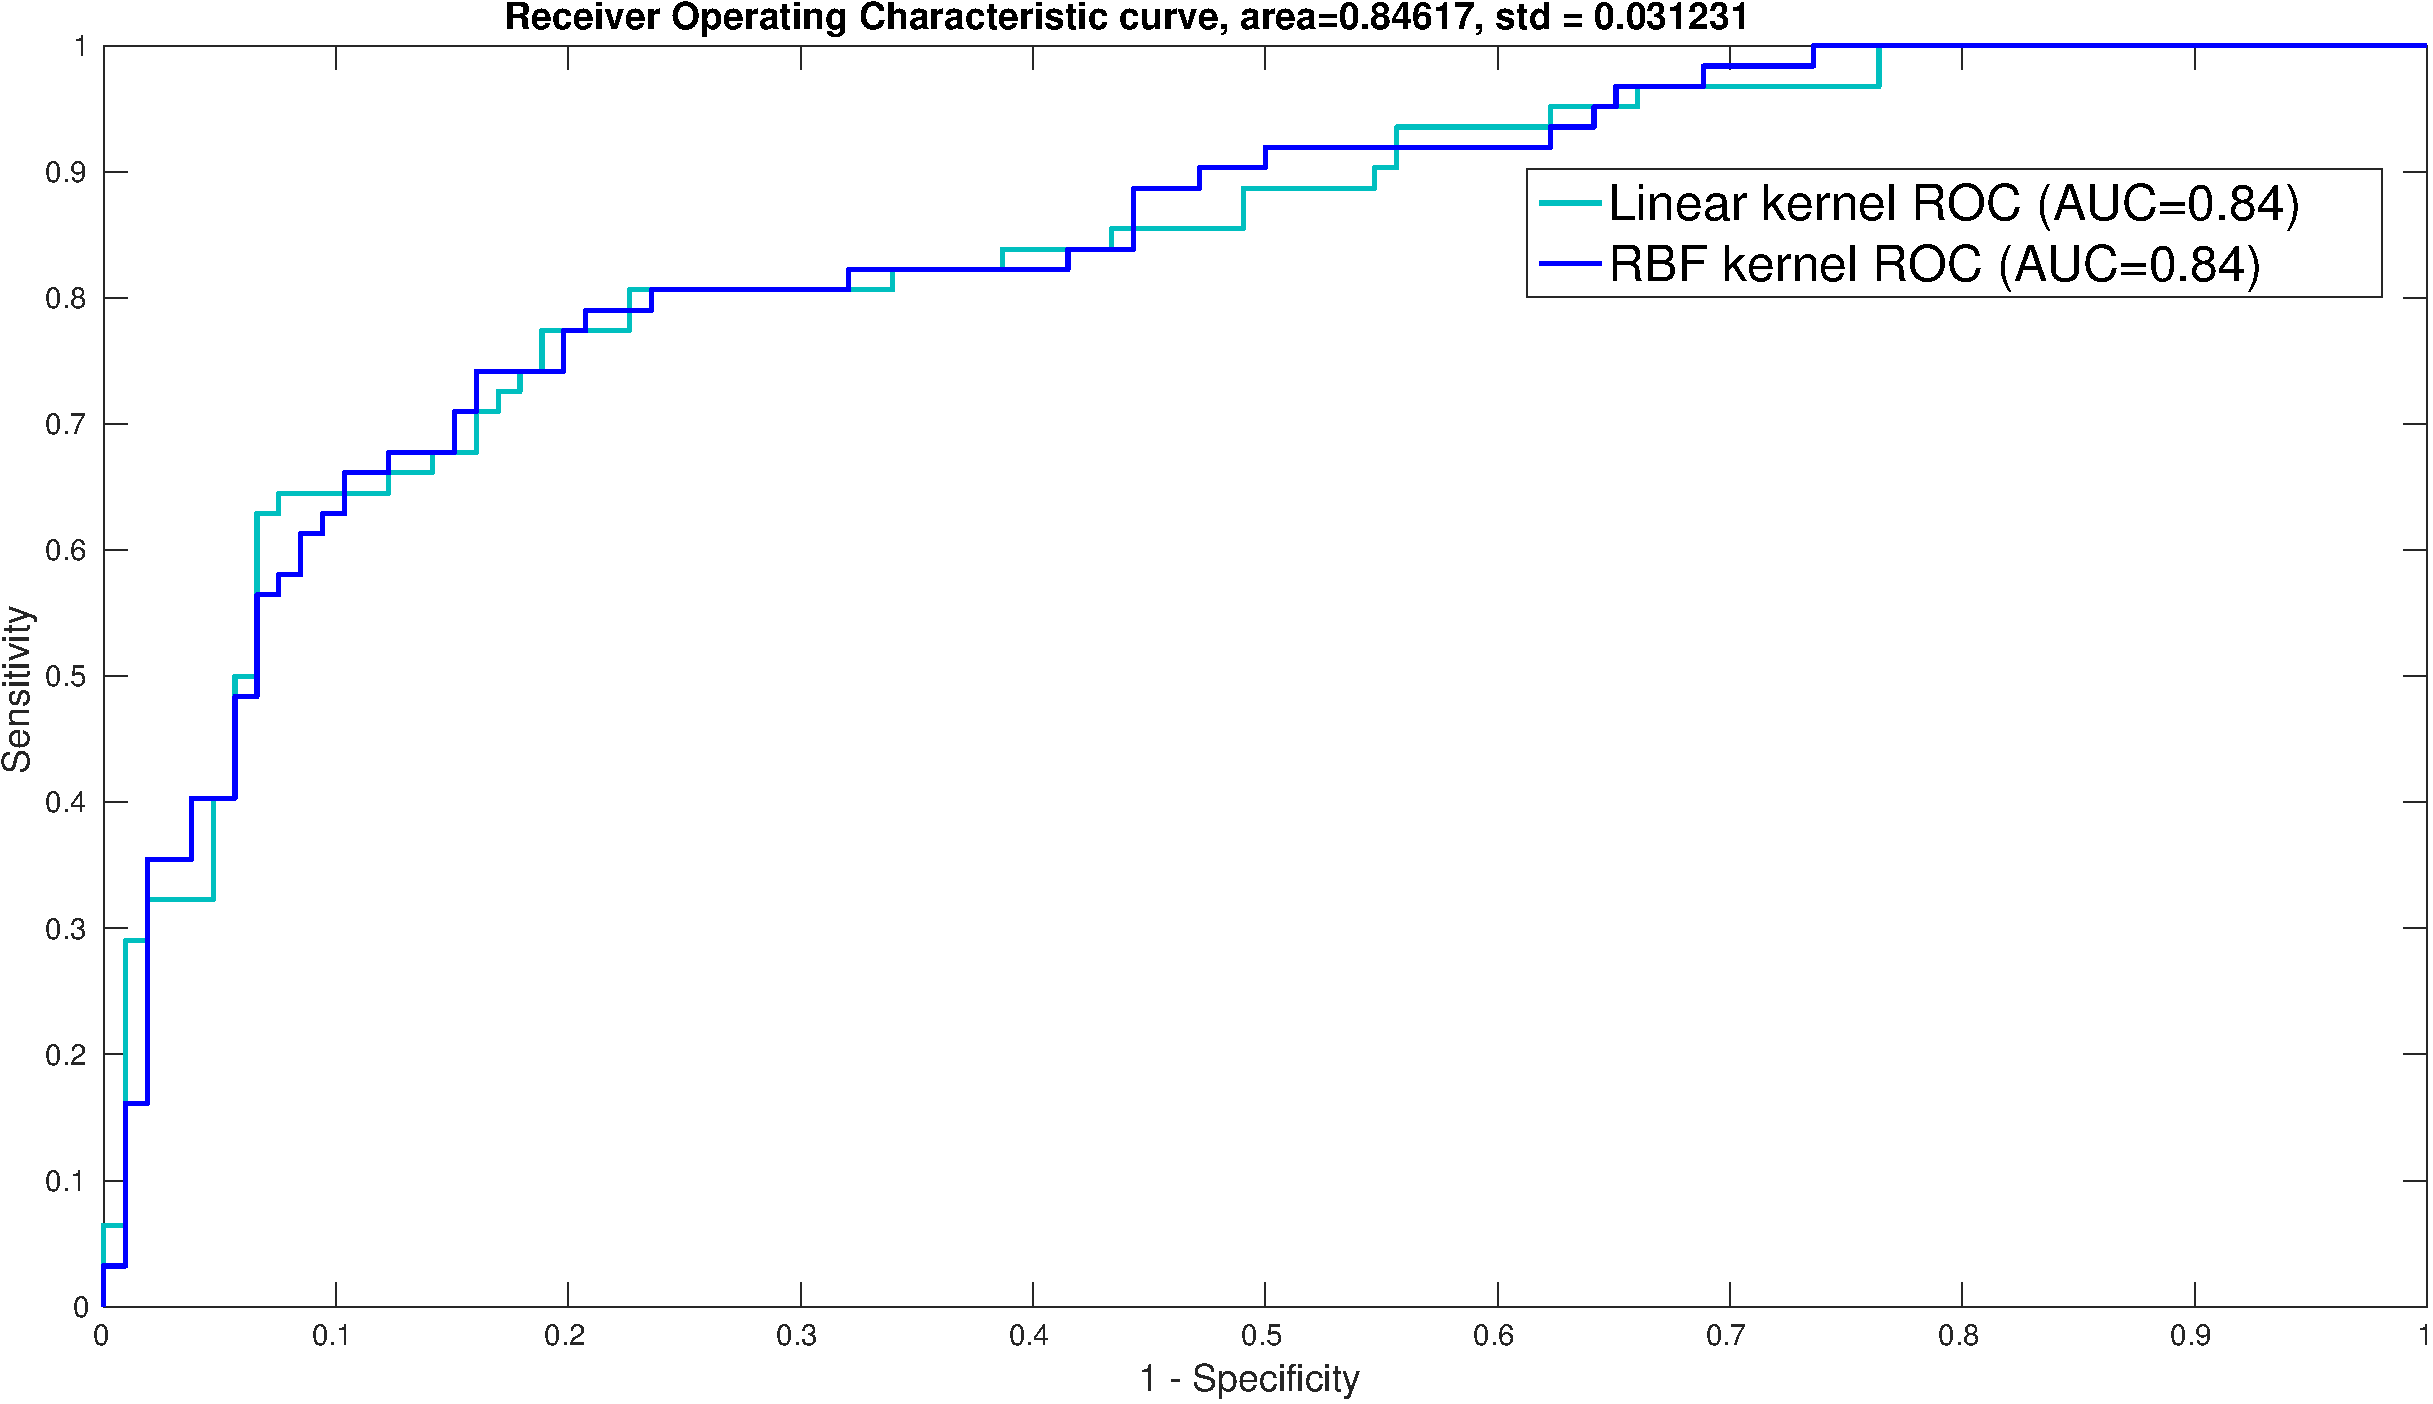
\includegraphics[scale=.40]{diabetes_ROC.pdf}
    \caption{ROC of both classifiers}
    \label{fig:diabetes_ROC}
\end{figure}

\subsubsection{Final model selection}

For this dataset, the performances are slightly worse than we had for
the previous ones. I couldn't see evidences of linear separability in
the PCA plot with 3 PC, but that does not exclude that one exists. The
performance of both kernels are very similar, so I would advise to go
with the simplest method, which is the linear kernel.

%\bibliographystyle{ieeetr} \bibliography{bib-db}
\end{document}
